\documentclass{article}
\usepackage{float}
\usepackage{graphicx}
\usepackage{tabularx,booktabs}
\usepackage{caption}
\usepackage{subfig}
\usepackage{lipsum}
\usepackage{tikz}
\usepackage{eso-pic}
\usepackage{changepage}
\usepackage{xcolor}
\usepackage{afterpage}
\usepackage[document]{ragged2e}
\usepackage[none]{hyphenat}
\usepackage[margin=1in,footskip=0.25in]{geometry}
\usepackage{array}
% \usepackage{l3kernel}
% \usepackage{l3packages}
\usepackage{siunitx}
\usepackage{color,soul}
\usepackage{placeins}
\usepackage{microtype}
% \usepackage[backend=biber]{biblatex}
\usepackage[hidelinks]{hyperref}
\usepackage[toc,page]{appendix}
%\usepackage[toc]{glossaries}
\usepackage[subfigure]{tocloft}
\usepackage{rotating}
\usepackage[printwatermark]{xwatermark}
\usepackage{amssymb}
\usepackage[nottoc,notlof,notlot]{tocbibind} % Put the bibliography and index in the ToC
% \usepackage[table,xcdraw]{xcolor}
\hypersetup{
	colorlinks,
	linkcolor=[rgb]{0,0,0.50196},
	citecolor={blue!50!black},
	urlcolor={blue!80!black}
}

\cftsetindents{subsection}{.25in}{.4in}

\usepackage[flushleft]{threeparttable}
\newcolumntype{C}[1]{>{\centering\let\newline\\\arraybackslash\hspace{0pt}}m{#1}}

\definecolor{ULred}{HTML}{872434}

\usepackage{chngcntr}
\counterwithin{table}{section}
\counterwithin{figure}{section}

\pdfoptionpdfminorversion=6
%\addbibresource{FireAttackReport.bib}

\setlength{\parskip}{1em}

% ******* REMOVE COMMENTS AND PLACE GLOSSARY.TEX IN ROOT DIRECTORY TO ADD GLOSSARY, SEE END FOR ADDITIONAL LINES TO UNCOMMENTS *******
%
%\loadglsentries{glossary.tex}
%
%\makeglossaries

% ******* REMOVE COMMENTS ON THIS BLOCK TO ADD DRAFT TO REPORT ********
% \newsavebox\mybox
% \savebox\mybox{\tikz[color=gray,opacity=0.5]\node{DRAFT};}
% \newwatermark*[
% allpages,
% angle=65,
% scale=15,
% xpos=-65,
% ypos=20
% ]{\usebox\mybox}

\begin{document}
\bibliographystyle{unsrt}
	
	\begin{titlepage}
		
		\pagecolor{ULred}\afterpage{\nopagecolor}
		

		\AddToShipoutPictureFG*{\AtPageUpperLeft{\raisebox{-\height}{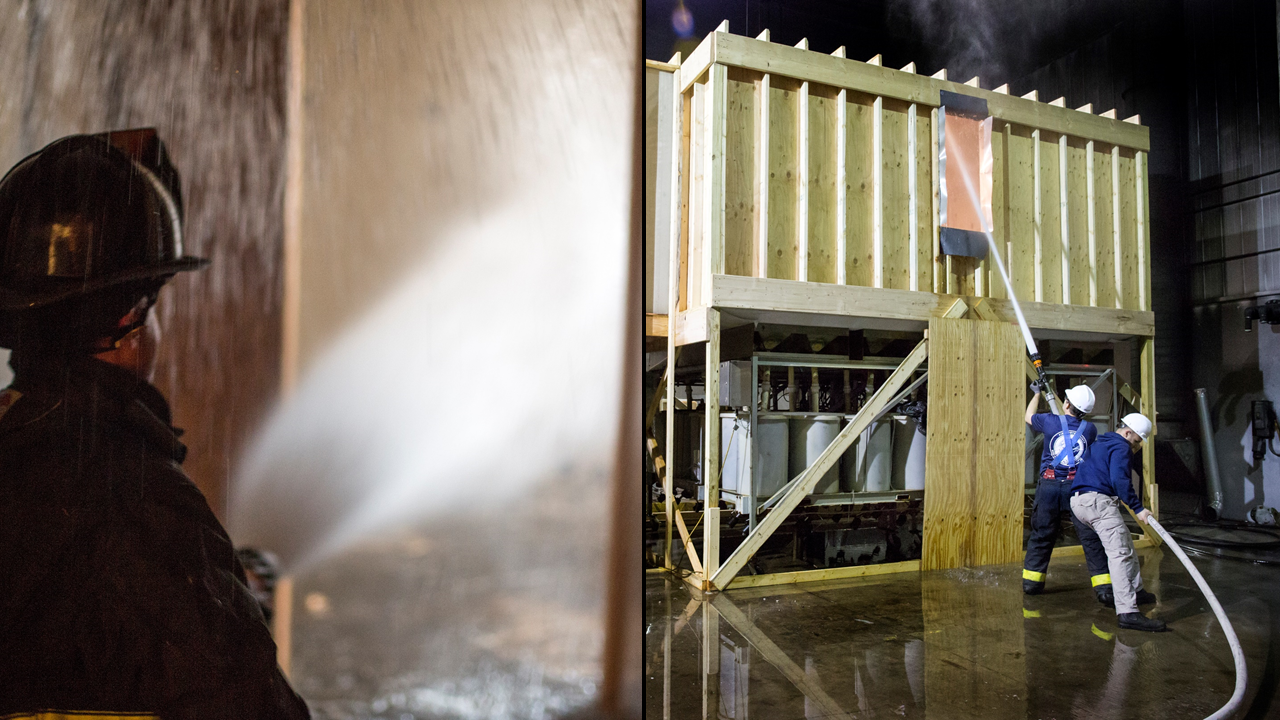
\includegraphics[width=7in]{Figures/General/TitlePagePhotoNew}}}} 

			\vspace*{20\baselineskip} 

		\huge
		\begin{adjustwidth}{-0.5in}{-0in}
		\color{white}
		\textbf{Study of the Impact of Fire Attack \\ Utilizing Interior and Exterior Streams \\ on Firefighter Safety and Occupant Survival}
		\end{adjustwidth}
		\huge
		\begin{adjustwidth}{-0.5in}{-0in}
		\color{white}
		\textbf{Water Distribution}
		\end{adjustwidth}
		\begin{adjustwidth}{-0.5in}{}
		\color{white}
		\vspace{.2\baselineskip}
		\large
		Keith Stakes \\
		Robin Zevotek \\
		UL Firefighter Safety Research Institute \\
		\vspace*{4\baselineskip}

		Stephen Kerber \\
		Director \\
		UL Firefighter Safety Research Institute \\

		\vspace*{.8\baselineskip}	
		\today
		\vspace*{.8\baselineskip}
		\begin{figure}[h]
			\hspace*{-0.5in}
\includegraphics[width=0.75in]{Figures/General/ULLogoWhite.pdf}
		\end{figure}
		\end{adjustwidth}
	\end{titlepage}

\begin{center}
	DISCLAIMER\\
	\vspace*{\baselineskip}
	\begin{adjustwidth}{-0.25in}{-0.25in}
		In no event shall UL be responsible to anyone for whatever use or non-use is made of the information contained in this Report and in no event shall UL, its employees, or its agents incur any obligation or liability for damages including, but not limited to, consequential damage arising out of or in connection  with the use or inability to use the information contained in this Report. Information conveyed by this Report applies only to the specimens actually involved in these tests. UL has not established a factory Follow-Up Service Program to determine the conformance of subsequently produced material, nor has any provision been made to apply any registered mark of UL to such material. The issuance of this Report in no way implies Listing, Classification or Recognition by UL and does not authorize the use of UL Listing, Classification or Recognition Marks or other reference to UL on or in connection with the product or system.
	\end{adjustwidth}
\end{center}

\begin{center}
	ACKNOWLEDGEMENTS
\vspace*{\baselineskip}
\begin{adjustwidth}{-0.25in}{-0.25in}
This work was funded through a grant from the Department of Homeland Security's Assistance to Firefighters Grant Program under the Fire Prevention and Safety Grants: Research and Development. Without this critical funding and support, this vital fire service research would not be possible.

\vspace*{\baselineskip}

\begin{center}
	
\includegraphics[width=0.28\textwidth]{Figures/General/DHS}
\end{center}

\clearpage

To assist the design and implementation of the experiments for the Fire Attack study, fire service experts were gathered from across the world with knowledge in fire suppression and the impact of interior and exterior fire streams. The individuals below provided direction for the project, assisting in planing the experiments, witnessing the testing, and developing concrete conclusions. Their tireless support and effort make this project relevant to the fire service across the world. 

\vspace*{\baselineskip}

\renewcommand{\arraystretch}{1.5}

\begin{table}[H]
	\centering
	\caption*{Fire Service Technical Panel}
	\begin{tabular}{ll}
		\toprule[1.5pt]
		Name & Fire Department \\ 
		\midrule
		Steve Brisebois  & Montreal Fire Department \\ 
		Matt Carrigan    & Montgomery County Fire and Rescue Service \\ 
		Tony Carroll     & Washington DC Fire Department \\ 
		Albert Castillo  & Houston Fire Department \\ 
		Chad Christensen & Los Angeles County Fire Department \\ 
		John Chubb       & Dublin Fire Brigade \\ 		 		  
		Danny Doyle      & Pittsburgh Fire Department \\ 
		Aaron Fields     & Seattle Fire Department \\ 
		Jason Floyd      & Las Cruces Fire Department \\ 
		John Gallagher   & Boston Fire Department \\ 
		Chad Green       & Anchorage Fire Department \\ 
		Kelly Hanink     & Eden Prairie Fire Department \\ 
		Samuel Hittle    & Wichita Fire Department \\ 
		Jacob Hoffman    & Toledo Fire/Rescue Department \\ 
		Josh Hummel      & Howard County Department of Fire and Rescue Services \\ 
		Jerry Knapp      & West Haverstraw (NY) Fire Department \\ 
		Dennis Legear    & Oakland Fire Department \\ 
		Hans Neiling     & Zuid Limburg Fire \\ 
		Nick Martin      & Columbia Fire Department \\ 
		Ray McCormack    & Fire Department of New York \\ 
		John McDonough   & New South Wales Fire Department \\ 
		Jordan Mohr      & Sedgwick County Fire District 1 \\ 
		Steve Pegram     & Goshen Township Fire and EMS \\ 
		\bottomrule[1.25pt]
	\end{tabular}
\end{table}

\end{adjustwidth}
\end{center}

\clearpage

\renewcommand{\abstractname}{Abstract}
\setlength{\emergencystretch}{5pt}

\begin{abstract}

As research continues into how fire department interventions affect fire dynamics in the modern fire environment; questions continue to arise on the impact and implications of interior versus exterior fire attack on both firefighter safety and occupant survivability. Previous research into various types of fire ground ventilation, flow paths, and exterior fire streams has provided the fire service with a more in-depth understanding of fire dynamics in addition to causing concern about certain fire attack methods stemming from differing traditions and myths. This knowledge gap and lack of previous research in this area has driven the need for further study into fire department interventions at structure fires with a focus on hose streams and suppression tactics. Statistics show that both firefighters and building occupants continue to loose their lives due to fire. As such, research into the various methods of fire attack will allow a broader understanding of how firefighter interventions on the fire ground can impact the outcome of both life safety and property protection. 

\vspace*{\baselineskip}

This study will build and expand upon the fire research conducted to date by analyzing how firefighting tactics, specifically suppression methods, affect the thermal exposure and survivability of both firefighters and building occupants in addition to impacting fire behavior in structures. The purpose of this study is to improve firefighter safety, fireground tactics, and the knowledge of fire dynamics by providing the fire service with credible scientific information, developed from both water flow and full-scale fire testing, in representative single family homes. The project will be comprised of 3 parts:
\vspace*{\baselineskip}
\begin{itemize}
	\item Part I:  Water Distribution
	\item Part II: Air Entrainment
	\item Part III: Full-Scale Residential Fire Experiments
	\end{itemize}
\vspace*{\baselineskip}

This report details the results and analysis from the water distribution experiments. These tests were conducted without the presence of fire to gain a fundamental understanding of water flow the remaining parts of the study were conducted. Each test was designed to quantify water distribution within compartments by evaluating the differences caused by various application methods, hose stream types, nozzle movements, pressures/flow rates, and stream locations and elevation angles. 

\end{abstract}

\newpage

\tableofcontents

\newpage

\section{Background}

Recent fire service research has highlighted the importance of applying water to the fire as quickly as possible. This tactical consideration has highlighted a knowledge gap and increased the interest in better understanding the impact of water applied as part of an interior or exterior attack. Many variables exist in fire attack that impact firefighter effectiveness and victim survivability including stream placement, the time required to get water on the fire, stream type, stream movement, air entrainment, steam development, hot gas cooling and contraction, and position of flow paths. The most important firefighting tool for many years at structure fires has been their hoseline; however, many questions have arisen as more research shows the impact of ventilation, flow paths, and exterior fire streams. Whether a fire attack crew chooses to apply water as part of an interior attack or as part of an exterior or ``transitional attack," they need to know what impact their stream has on the fire environment ahead of them. This is difficult on the fire ground because visibility is commonly limited and therefore most experience and first-hand accounts are from behind the nozzle. This results in beliefs about conditions (e.g. temperature) ahead of the nozzle team and the impact of their tactics on victim survivability; but knowledge of the actual impact has yet been researched. Additionally, when the fire is ultimately suppressed, there is no assurance the attack was conducted in the most effective, efficient, and safe manner even if the experience gained suggests that it was. Fire service adages such as ``don’t put water on smoke,'' ``you will steam the victims,'' and ``fog nozzles always disrupt the thermal layer'' have been passed on from generation to generation with little context or substantiation. Without the context, these concepts get treated like rules and can severely limit firefighters understanding of fire suppression.

Current fire training curriculum defines 3 fire attack methods: direct attack, indirect attack, and combination attack. Direct attack involves the discharge of water directly onto the burning fuel. Indirect attack involves directing the stream toward the ceiling of a compartment in order to generate a large amount of steam in order to cool the compartment. Converting the water to steam displaces oxygen, absorbs the heat of the fire and cools the hot gas layer sufficiently for firefighters to safely enter and make a direct attack. Combination attack extinguishes a fire by using both a direct and indirect attack. Another technique to safely approach a fire that cannot be reached with a direct attack is gas cooling. Gas cooling provides a buffer zone around the attack team but the larger the compartment, the less the impact on cooling the hot gas layer. Gas cooling must be a continuous process while advancing toward a shielded fire. Techniques for effective gas cooling and the upper limit of the volume where gas cooling is effective is not well known.  

\hl{*** ADD BACKGROUND SPECIFIC TO AIR ENTRAINMENT AND ADD ***}
\hl{DAN TO ORGANIZE}

Fire suppression effectiveness and firefighter safety are not achieved by water flow rate alone, but by appropriate use of a given flow rate under specific fire ground conditions. A flow rate must meet the critical flow rate to extinguish a fire depending on the heat release rate and should be higher to reduce the time to extinguishment. Drastically exceeding the critical flow rate has less known impact on time to extinguishment but has a significant impact on the total amount of water used. To-date, there is little data to connect the critical flow rate to firefighter safety. However, it has been estimated that only 5 to 10 percent of water applied during fire attack contributes to extinguishment. It is difficult for firefighters to realize the the efficiency of various hose stream techniques due to poor visibility on the fireground. However, by developing data in realistic structures, fuel sources, and fire scenarios, important inferences may be developed relative to different hose stream techniques, and use of water.

\clearpage

\section{Objectives}

\subsection {Objectives}

The purpose of this part to the overall study was to provide the fire service with scientific based knowledge on the impact of hose streams during interior and exterior fire attack on firefighter safety and trapped occupants to improve training and decision making on the fire ground. This was accomplished with the completion of the following objectives:

\begin{itemize}
	\item Improve firefighter safety by increasing knowledge of fire suppression.
	\item Develop knowledge of hose streams applied during an interior and exterior fire attack and its impact on firefighter safety and victim survivability.
	\item Understand where water goes and how air flows during interior and exterior fire attack utilizing common equipment, practices, and tactics.
	\item Gain understanding of the impact of water streams depending on the volume of the fire compartment/structure.
	\item Bring the `Science to the Streets' by transferring science based conclusions founded on experimental results that can be incorporated into firefighting standard operating procedures.
	\end{itemize}

\clearpage


\section{Water Distribution Experiments}

The goal of the water distribution experiments was to quantify the impact that changing a nozzle, changing flow pressure, or changing flow position had on water dispersion within a compartment. Eighty-four water flow tests were conducted at the UL Headquarters in Northbrook, IL in a purpose built compartment with an attached hallway and movable staircase. Water flow patterns were determined by collecting the water in 48 discrete collection bins. A detailed description of the water collection is in Section~\ref{sec:add_instrumentation}.

\subsection{Experimental Configuration}

\subsubsection{Test Apparatus}
\label{ADD_discussion}
The main portion of test compartment had interior (finished) dimensions of 14~ft 8~in. by 10~ft 5~in with an 8~ft ceiling. To account for water collection apparatus the entire compartment was 7~ft 11~in above the floor of the lab floor (see Figure~\ref{fig:Water_Distribution_Test_Structure_and_ADD_Apparatus}). The overall size of the compartment was designed to reflect that of one found in a typical resident structure but was also bound by the dimensions of the water collection apparatus (Section~\ref{sec:add_instrumentation}). The compartment was wood frame construction with 2~in. by 4~in. studs and track set to 16~in. centers with a interior height measuring 8~ft 1 1/8~in. rough. The walls and ceiling were lined with 1/2~in. durarock cement board atop 1/2~in. plywood. The ceiling joists were 2~in. by 6~in. set to 16~in. on center.

\begin{figure}[!ht]
	\centering
	\includegraphics[width=.8\columnwidth]{Figures/Water_Distribution/Building.jpg}
	\caption{Water Distribution Test Structure and ADD Apparatus}
	\label{fig:Water_Distribution_Test_Structure_and_ADD_Apparatus}
\end{figure}

The compartment featured two ventilation openings, one doorway measuring 3~ft by 6~ft 8~in. which opened to the interior hallway, and one window measuring 2~ft by 4~ft which opened to the exterior of the compartment. A movable staircase and landing was constructed to provide access to either the interior hallway of the compartment or provide a simulation of a first floor exterior attack. The hallway was 6~ft by 8~ft and the stairway landing was 4~ft by 6~ft 8~in. Detailed dimension drawings of the compartment are included in Figures~\ref{fig:ADD_Top_View} and \ref{fig:ADD_Side_View}

\begin{figure}[!ht]
	\centering
	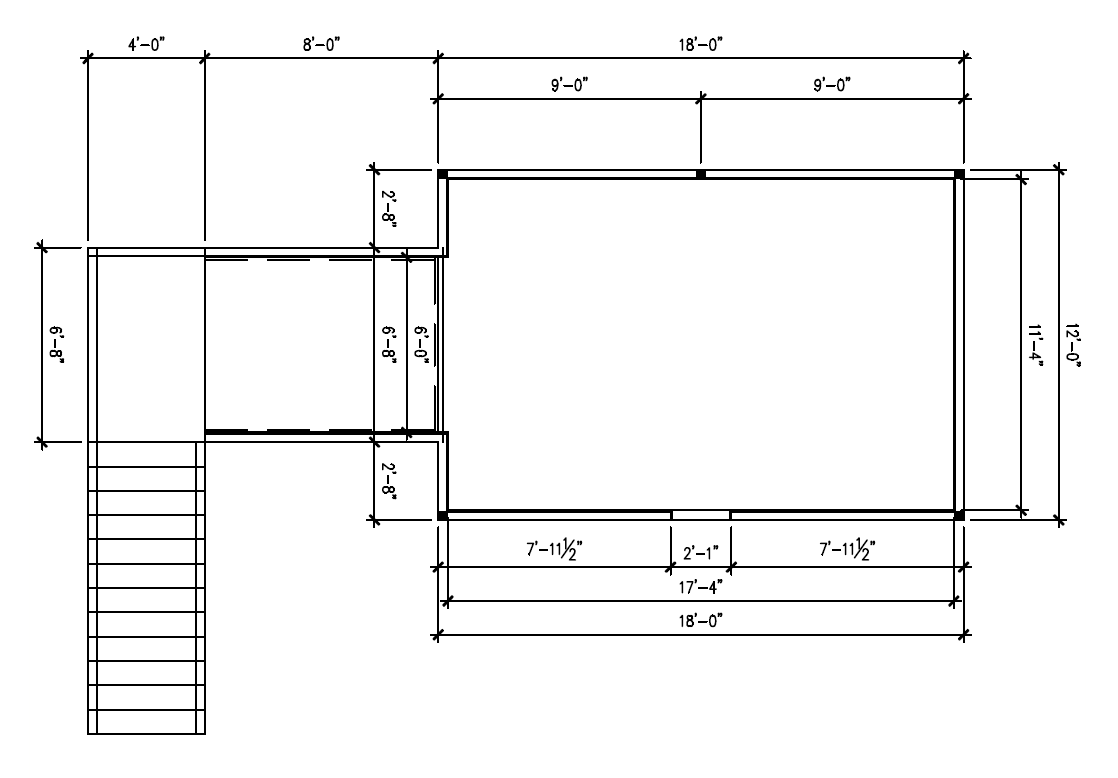
\includegraphics[width=\columnwidth]{Figures/Water_Distribution/ADDtopviewprint}
	\caption{ADD Plan View}
	\label{fig:ADD_Top_View}
\end{figure}

\begin{figure}[!ht]
	\centering
	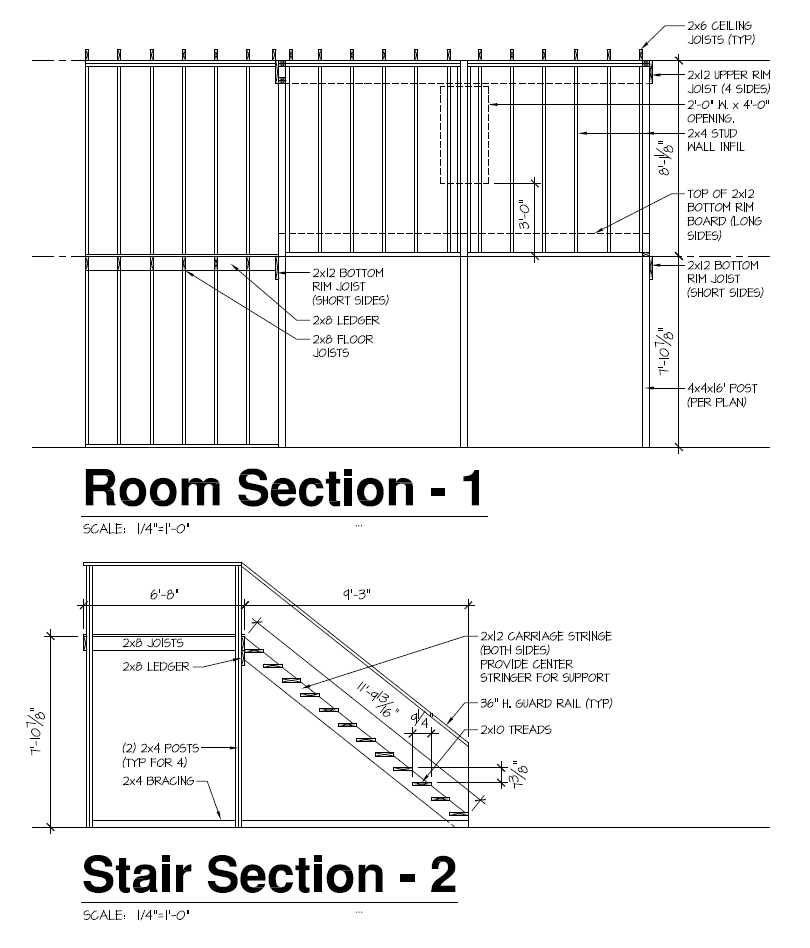
\includegraphics[width=\columnwidth]{Figures/Water_Distribution/ADDsideviewprint}
	\caption{ADD Section View}
	\label{fig:ADD_Side_View}
\end{figure}

\clearpage

A unique feature of this compartment was that there was no floor constructed. The test compartment instead sat directly over 48, 20~in by 20~in stainless steel collection bins. Instead of water accumulating on the floor, in would flow into the distinct collection bins to determine accumulation. Potential gaps between the collection bins were covered by flashing which was folded to divert the water evenly in each bin, to best ensure adequate distribution results. The gaps between the outer collection bins and the walls of the structure were also covered with flashing to ensure all water directed into the structure was collected in the appropriate bins. The interior layout of the floor bins and use of flashing can be seen in Figure \ref{fig:ADD_Flashing}. 

\begin{figure}[!ht]
	\centering
	\includegraphics[width=.7\columnwidth]{Figures/Water_Distribution/floor3.jpg}
	\caption{Layout of Structure Floor with 48 Collection Bins and Connected Flashing}
	\label{fig:ADD_Flashing}
\end{figure}

\subsubsection{Instrumentation and Uncertainty}
\label{sec:add_instrumentation}

To measure the water distribution throughout the compartment, a fire sprinkler spray density measurement instrument known as the Actual Delivered Density (ADD) apparatus was used. This device was connected to the 48 collection bins that comprised the floor of the test structure. The ADD apparatus is comprised of one main array and two satellite arrays of heavy steel framework. The main array consists of 32 water barrels and water pan collection assemblies while each satellite array contains 8 barrels and collection assemblies (see Figure~\ref{fig:ADD_Collection_Assembly}. All barrels are of 30-gallon capacity and are connected by a 2~in. diameter hose to a 20~in. by 20~in. inverted square pyramid shaped stainless steel water collection pan above. In total, there are 48 total collection pans/barrels. Differential pressure transducers connect to the bottom of each water collection barrel via flexible tubing. The water level in a given barrel is determined by the head pressure measured by the transducer. The water collection rate is calculated based the change in head pressure over time. As Figure \ref{fig:Bin Numbers and Locations} shows, collection assemblies were arranged into 2~$\times$~2 arrays. Each collection barrel is uniquely numbered so that water flow data can be mapped to specific position. The barrels are connected to a pneumatic drain valve which could be actuated to drain each barrel at the conclusion of an experiment. 

\begin{figure}[!ht]
	\centering
	\begin{tabular}{cc}
		\subfloat[Collection Barrels]{\includegraphics[height = .3\columnwidth]{Figures/Water_Distribution/ADD2.jpg}} &
		\subfloat[Collection Pans]{\includegraphics[height = .3\columnwidth]{Figures/Water_Distribution/ADDbottom3.jpg}} \\
	\end{tabular}
	\caption{ADD Collection Assembly}
	\label{fig:ADD_Collection_Assembly}
\end{figure}

\begin{figure}[!ht]
	\centering
	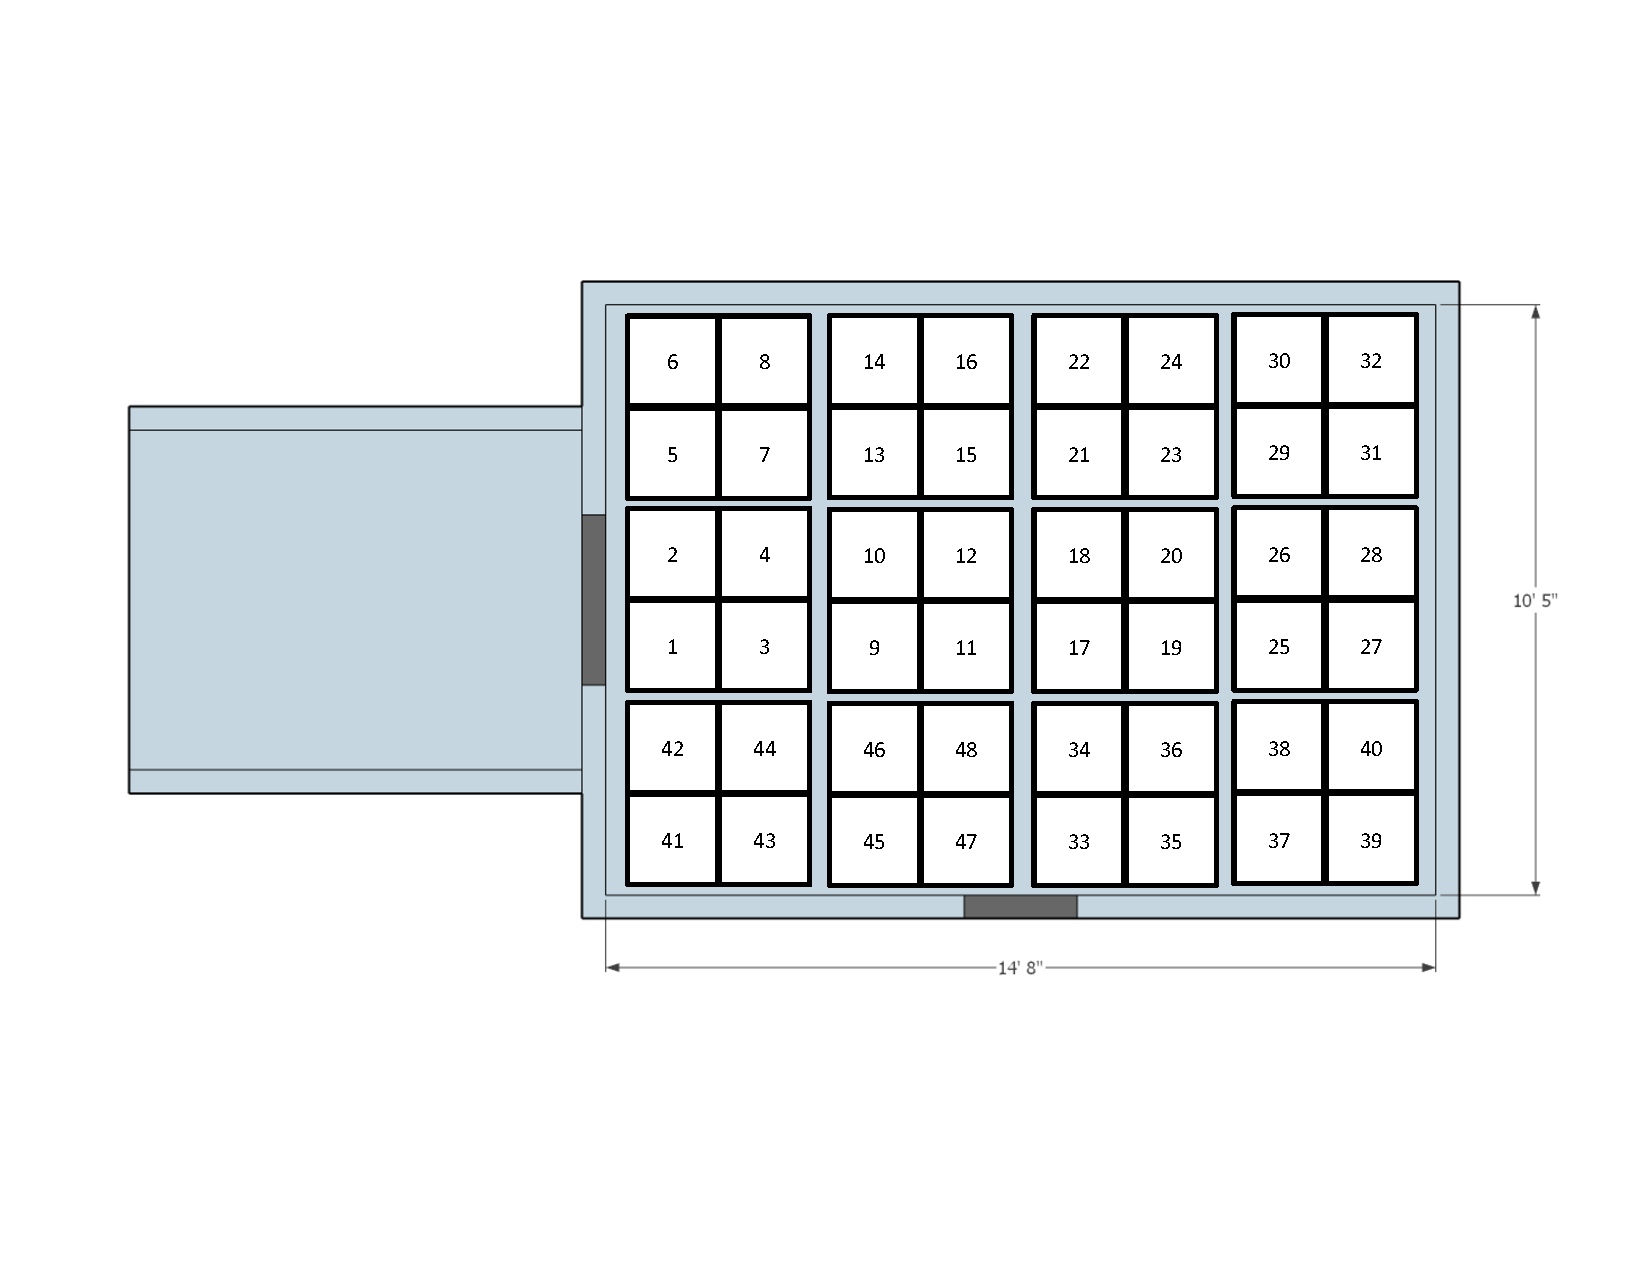
\includegraphics[width=\columnwidth]{Figures/Water_Distribution/Bin_Numbers_NoDimensions}
	\caption{Bin Numbers and Locations}
	\label{fig:Bin Numbers and Locations}
\end{figure}

Prior to testing, data was collected to estimate the uncertainty associated with the water distribution measurements performed using the ADD apparatus. Each water collection assembly was filled to capacity while recording pressure transducer measurements as well as data from a calibrated turbine flowmeter (with less than 1~\% measurement uncertainty). Although the design of each water collection assembly is the same, the measurement performance across the entire apparatus varied. Overall, the 48 water collection assemblies reported an average accuracy of $\pm$ 2.4~gallons. This represents an uncertainty in total volume of $\pm$ 8~\% at full scale (30 gal).

\subsubsection{Experimental Equipment}

To ensure the data collected were applicable to the majority of the fire service, a representative set of nozzles types, specified flows/pressures, and hose sizes were used. These test variables are similar to those discussed in the air entrainment experiments and are shown in Table~\ref{tab:nozzles_used_detail}.

\begin{table}[!ht]
\centering
\caption{Primary Equipment Configurations}
\label{tab:nozzles_used_detail}
\begin{tabular}{llccc}
\toprule[1.5pt]
Line Size & Nozzle Type & Tip (in) & Nozzle Pressure (psi) & Approximate Flow Rate (gpm) \\ 
\midrule
1 3/4 in. & Smooth Bore          & 1      & 50 & 210 \\
          & Smooth Bore          & 15/16  & 50 & 180 \\
          & Smooth Bore          & 7/8    & 50 & 150 \\
          & Combination          &        & 100 & 100 \\
          & Combination          &        & 100 & 150 \\
          & Combination          &        & 75 & 150 \\
          & Combination          &        & 50 & 150 \\ \midrule
2 1/2 in. & Smooth Bore          & 1 1/4  & 50 & 260 \\
          & Combination          &        & 100 & 250 \\
\bottomrule[1.25pt]
\end{tabular}
\end{table}

\subsection{Experiments Conducted}

The water distribution experiments consisted of 84 tests that incorporated both interior and exterior fire attack utilizing the various nozzles and flow configurations. In each test, water flowed for approximately 1~min. in duration. The duration was dictated by the size of the collection barrels in the ADD apparatus. Each collection barrel was a total of 30 gallons. If a barrel overflowed, there would be an inability to determine the correct distribution of water flow. At the start of each test, there was an initial amount of water in the bottom of the barrel to ensure the sensors were able to record the water received during the testing. The total water in each barrel was determined by subtracting the initial water volume in each barrel from the final value. 

\subsubsection{Interior Tests}
\label{int_tests}
The interior tests were designed to simulate a fire on the same floor as the attack crew. Suppression operations were conducted from the doorway adjoining the hallway to the test compartment. At this location, hose stream type, nozzle direction, and spray pattern were varied and the water distribution within the compartment was measured. The three nozzle directions, max angle ceiling, mid ceiling, and at wall are shown in Figure \ref{fig:Nozzle_Direction_Interior_Attack}. The max angle ceiling position was defined to be the steepest angle the nozzle could be without the stream being impacted by the soffit of the doorway. The mid ceiling position set the stream to hit the middle of the ceiling along the 14~ft 8~in. dimension. The third position, the wall position, was defined to have the stream hit the vertical midpoint of the wall adjacent to the doorway. Table~\ref{tab:Interior_Fire_Attack_Distribution_Experiments} lists the interior tests conducted.

\begin{figure}[!ht]
	\centering
	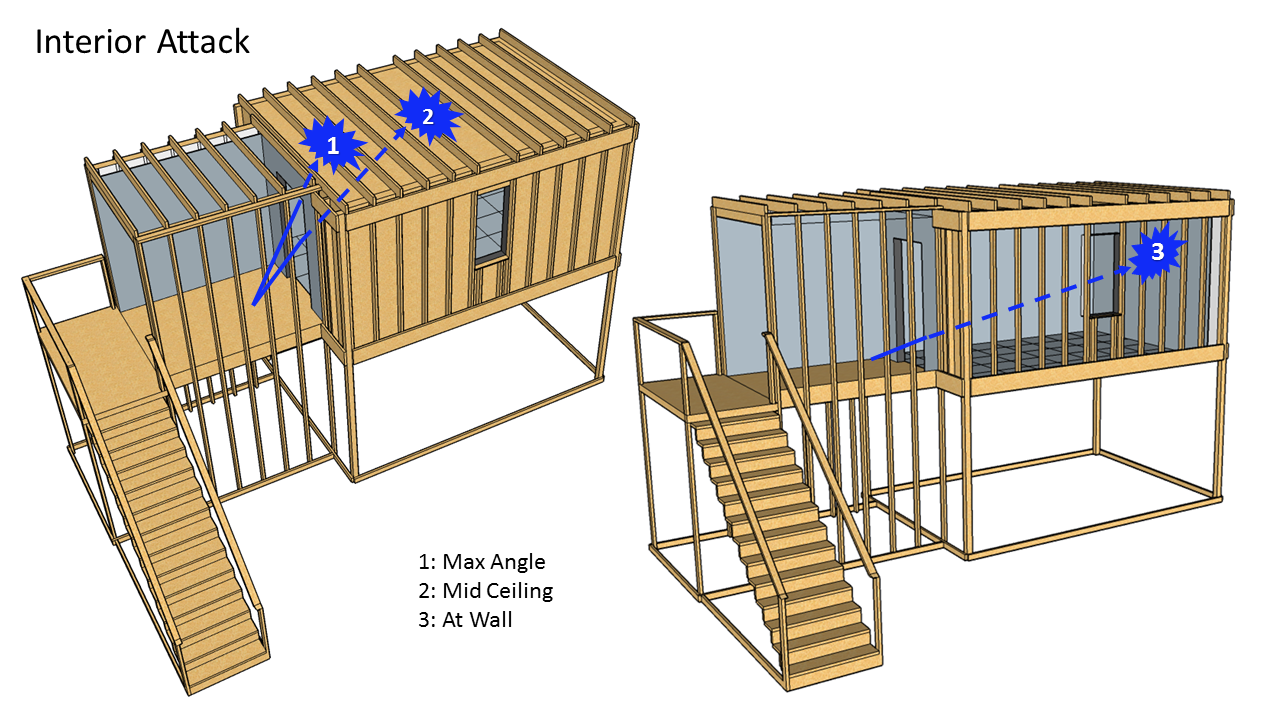
\includegraphics[width=\columnwidth]{Figures/Water_Distribution/Nozzle_Position_Int}
	\caption{Nozzle Direction, Interior Attack}
	\label{fig:Nozzle_Direction_Interior_Attack}
\end{figure}

\begin{table}[]
\centering
\small
\caption{Interior Water Distribution Experiments}
\label{tab:Interior_Fire_Attack_Distribution_Experiments}
\begin{tabular}{ccccc}
\toprule[1.5pt]
Hose Stream Type & Nozzle Direction & Nozzle Movement & Nozzle Pressure (psi) & Flow Rate (gpm) \\ 
\midrule
Straight Stream   & Max Angle Ceiling   & O       & 100 & 150 \\
Straight Stream   & Max Angle Ceiling   & Fixed   & 100 & 150 \\
Straight Stream   & Mid Ceiling 		& Fixed   & 100 & 125 \\
Straight Stream   & Mid Ceiling 		& O       & 100 & 125 \\
Straight Stream   & Mid Ceiling 		& Z       & 100 & 125 \\
Straight Stream   & Mid Ceiling 		& T       & 100 & 125 \\
Straight Stream   & Mid Ceiling 		& Inverted U & 100 & 125 \\
Straight Stream   & Mid Ceiling 		& Fixed   & 100 & 150 \\
Straight Stream   & Mid Ceiling 		& O       & 100 & 150 \\
Straight Stream   & Mid Ceiling 		& Fixed   & 75 & 150 \\
Straight Stream   & Mid Ceiling 		& O & 75  & 150 \\
Straight Stream   & Mid Ceiling 		& Fixed   & 50 & 150 \\
Straight Stream   & Mid Ceiling 		& O & 50  & 150 \\
Straight Stream   & At Wall     		& Fixed   & 100 & 150 \\
Straight Stream   & At Wall     		& O       & 100 & 150 \\
Fog               & Mid Ceiling 		& Fixed   & 100 & 125 \\
Fog               & Mid Ceiling 		& Fixed   & 100 & 150 \\
Fog               & Mid Ceiling 		& O       & 100 & 150 \\
Fog               & Mid Ceiling 		& Fixed   & 75 & 150 \\
Fog               & Mid Ceiling 		& O & 75  & 150 \\
Fog               & Mid Ceiling 		& Fixed   & 50 & 150 \\
Fog               & Mid Ceiling 		& O & 50  & 150 \\
Fog               & Mid Ceiling 		& O       & 100 & 125 \\  
15/16 Smooth Bore & Max Angle Ceiling   & Fixed   & 50 & 180 \\
15/16 Smooth Bore & Max Angle Ceiling   & O & 50  & 180 \\
15/16 Smooth Bore & At Wall     		& Fixed   & 50 & 180 \\
15/16 Smooth Bore & At Wall     		& O & 50  & 180 \\
15/16 Smooth Bore & Mid Ceiling 		& Fixed   & 50 & 180 \\
15/16 Smooth Bore & Mid Ceiling 		& O & 50  & 180 \\
\bottomrule[1.25pt]
\end{tabular}
\end{table}

\clearpage

\subsubsection{Exterior Tests}
\label{ext_tests}

The exterior testing included two attack positions; one attack was from the fire floor and the second was from the floor below the fire. These are referred to as first floor and second floor attacks. The movable staircase to allowed for the variation between first floor and second floor suppression through the same window vent. The exterior tests simulated a single room of fire in which an exterior attack was used. Similar to the interior testing, the hose stream type, the nozzle direction, and application pattern were varied for comparison. The differences in first floor and second floor attacks can been seen in Figures \ref{fig:Nozzle_Direction_Exterior_1st_Floor_Attack} and \ref{fig:Nozzle_Direction_Exterior_2nd_Floor_Attack}. 

There were five nozzle directions for the first floor exterior tests: max angle ceiling, mid ceiling, min angle ceiling, max angle wall, and at wall. The max angle ceiling position was defined as the steepest angle the nozzle could be positioned at without the window soffit impacting the hose stream. The mid ceiling position was defined by the hose stream aimed at the center of the compartment in the 10~ft 5~in dimension. The min angle ceiling position was defined by the shallowest angle such the hose stream did not directly contact the wall. The max angle wall is similar to the max angle ceiling except it was defined as the steepest angle where the hose stream would impact the wall without the stream contacting the ceiling directly. The final position was aiming the stream at the position on the wall across from the window.

There were five nozzle directions for the second floor exterior tests: max angle ceiling, mid ceiling, min angle ceiling, max angle wall, and soffit. The first four positions were the same as the first floor exterior attack except that the starting position of the nozzle changed to be one story below the window vent. The fifth nozzle position, at soffit, was defined to be the maximum angle such that stream directed off the window soffit.

The exterior tests are shown in Table~\ref{tab:Exterior_Fire_Attack_Distribution_Experiments}.

\begin{figure}[!ht]
	\centering
	\includegraphics[width=\columnwidth]{Figures/Water_Distribution/Nozzle_Position_ExtFirstfloor}
	\caption{Nozzle Direction, Exterior 1st Floor Attack}
	\label{fig:Nozzle_Direction_Exterior_1st_Floor_Attack}
\end{figure}

\begin{figure}[!ht]
	\centering
	\includegraphics[width=\columnwidth]{Figures/Water_Distribution/Nozzle_Position_ExtSecondfloor}
	\caption{Nozzle Direction, Exterior 2nd Floor Attack}
	\label{fig:Nozzle_Direction_Exterior_2nd_Floor_Attack}
\end{figure}

\clearpage

\begin{table}[!ht]
\centering
\scriptsize
\caption{Exterior Water Distribution Experiments}
\label{tab:Exterior_Fire_Attack_Distribution_Experiments}
\begin{tabular}{lcccccl}
\toprule[1.5pt]
Floor & Hose Stream Type & Nozzle Direction & Nozzle Movement & Nozzle Pressure (psi) & Flow Rate (gpm) & Notes \\ 
\midrule

First  & Straight Stream  & Max Angle Ceiling      & Fixed              & 100 & 150 &   \\
First  & Straight Stream  & Max Angle Ceiling      & Fixed              & 100 & 150 &   \\
First  & Straight Stream  & Max Angle Ceiling      & Fixed              & 100 & 150 &   \\
First  & Straight Stream  & Max Angle Ceiling      & Fixed              & 100 & 150 &   \\
First  & Straight Stream  & Max Angle Ceiling      & Fixed              & 100 & 150 &   \\
First  & Straight Stream  & Max Angle Ceiling      & Fixed              & 100 & 150 &   \\
First  & Straight Stream  & Max Angle Ceiling      & Fixed              & 100 & 150 &   \\
First  & Straight Stream  & Max Angle Ceiling      & Fixed              & 100 & 150 & 1/2 Bail  \\
First  & Straight Stream  & Max Angle Ceiling      & Fixed              & 100 & 150 & 45~s Flow  \\
First  & Straight Stream  & Max Angle Ceiling      & Fixed              & 100 & 150 & 30~s Flow  \\
First  & Straight Stream  & Max Angle Ceiling      & Fixed              & 75  & 150 & 15~s Flow  \\
First  & Straight Stream  & Max Angle Ceiling      & Fixed              & 75  & 60 &   \\
First  & Straight Stream  & Max Angle Ceiling      & Fixed              & 50  & 185 &   \\
First  & Straight Stream  & Max Angle Ceiling      & Fixed              & 50  & 150 &   \\
First  & Straight Stream  & Max Angle Ceiling      & Fixed              & 25  & 150 &   \\
First  & Straight Stream  & Max Angle Ceiling      & Fixed              & 25  & 130 & 30~s Flow  \\
First  & Straight Stream  & Max Angle Ceiling      & Fixed              & 100 & 250 &   \\
First  & Straight Stream  & Max Angle Ceiling      & Sweeping           & 100 & 150 &   \\
First  & Straight Stream  & Max Angle Ceiling      & Wide Sweep         & 100 & 150 &   \\
First  & Straight Stream    & Mid Ceiling          & Fixed      		& 100 & 150 &   \\
First  & Straight Stream    & Min Angle Ceiling    & Fixed     		    & 100 & 150 &   \\
First  & Straight Stream    & Min Angle Ceiling    & Fixed      		& 100 & 250 &   \\
First  & Straight Stream    & Max Angle Wall       & Fixed     		    & 100 & 150 &   \\
First  & Straight Stream    & At Wall              & Fixed      		& 100 & 150 &   \\
First  & 15/16 Smooth Bore  & Max Angle Ceiling      & Fixed         	& 50 & 180 &   \\
First  & 15/16 Smooth Bore  & Max Angle Ceiling      & Sweeping      	& 50 & 180 &   \\
First  & 15/16 Smooth Bore  & Max Angle Ceiling      & Fixed        	& 50 & 180 & 1/2 Bail  \\
First  & 15/16 Smooth Bore  & Max Angle Ceiling      & Fixed        	& 30 & 150 &   \\
First  & 15/16 Smooth Bore  & Max Angle Ceiling      & Fixed        	& 15 & 130 &   \\
First  & 15/16 Smooth Bore  & Max Angle Ceiling      & Fixed        	& 10 & 100 &   \\
First  & 15/16 Smooth Bore  & Mid Ceiling            & Fixed 			& 50 & 180 &   \\
First  & 15/16 Smooth Bore  & Min Angle Ceiling      & Fixed			& 50 & 180 &   \\
First  & 15/16 Smooth Bore  & Max Angle Wall         & Fixed			& 50 & 180 &   \\
First  & 15/16 Smooth Bore  & At Wall                & Fixed 			& 50 & 180 &   \\
First  & 7/8 Smooth Bore    & Max Angle Ceiling      & Fixed         	& 50 & 150 &   \\
First  & 1 Smooth Bore      & Max Angle Ceiling      & Fixed        	& 50 & 210 &   \\
First  & 1 1/4 Smooth Bore  & Max Angle Ceiling      & Fixed         	& 50 & 260 &   \\
First  & Fog                & Max Angle Ceiling      & Fixed        	& 100 & 150 &   \\
First  & Straight Stream/Fog & Max Angle Ceiling    & Fixed/O           & 100 & 150 &   \\
\midrule
Second & Straight Stream    & Max Angle Ceiling      & Fixed                   & 100 & 150 &   \\
Second & Straight Stream    & Max Angle Ceiling      & Sweeping                & 100 & 150 &   \\
Second & Straight Stream    & Max Angle Ceiling      & Wide Sweep              & 100 & 150 &   \\
Second & Straight Stream    & Mid Ceiling            & Fixed                   & 100 & 150 &   \\
Second & Straight Stream    & Min Angle Ceiling      & Fixed                   & 100 & 150 &   \\
Second & Straight Stream    & Max Angle Wall         & Fixed                   & 100 & 150 &   \\
Second & Straight Stream    & Soffit         		 & Fixed                   & 100 & 150 &   \\
Second & 15/16 Smooth Bore  & Max Angle Ceiling      & Fixed                   & 50 & 180 &   \\
Second & 15/16 Smooth Bore  & Max Angle Ceiling      & Sweeping       	       & 50 & 180 &   \\
Second & 15/16 Smooth Bore  & Mid Ceiling            & Fixed                   & 50 & 180 &   \\
Second & 15/16 Smooth Bore  & Min Angle Ceiling      & Fixed                   & 50 & 180 &   \\
Second & 15/16 Smooth Bore  & Max Angle Wall         & Fixed                   & 50 & 180 &   \\
Second & 7/8 Smooth Bore    & Max Angle Ceiling      & Fixed                   & 50 & 150 &   \\
Second & 1 Smooth Bore      & Max Angle Ceiling      & Fixed                   & 50 & 210 &   \\
Second & Fog                & Max Angle Ceiling      & Fixed                   & 100 & 150 & 45~s Flow \\
Second & Fog                & Max Angle Ceiling      & Fixed/O                 & 100 & 150 &   \\
\bottomrule[1.25pt]
\end{tabular}
\end{table}

\clearpage

\subsection{Analysis \& Results}

The intent of the water flow testing was to determine the location of the water within the compartment as a function of several common fire service equipment configurations and application locations. Recall, the location of the water within the compartment was achieved using the ADD device (Section~\ref{sec:add_instrumentation}). To ensure that differences between water distributions within the compartment could be quantified, it was important to confirm the repeatability of the experimental setup. Four tests utilizing a straight stream nozzle flowing 150~gpm at 100~psi from a 1 3/4~in. hoseline from the exterior first floor position directed into the structure with a maximum angle were conducted to determine the variance in results. The total water in each of the 48 collection bins for the four replicate tests is shown in Figure~\ref{fig:Repeatability_Testing}. In the bar chart, bins with less than 8~gal. are colored blue, with more than 8~gal. but less than 16~gal. are colored green, with more than 16~gal. but less than 24~gal. are colored yellow, and bins with more than 24~gal. are colored red. 

\begin{figure}[ht]
\begin{tabular*}{\textwidth}{lr}
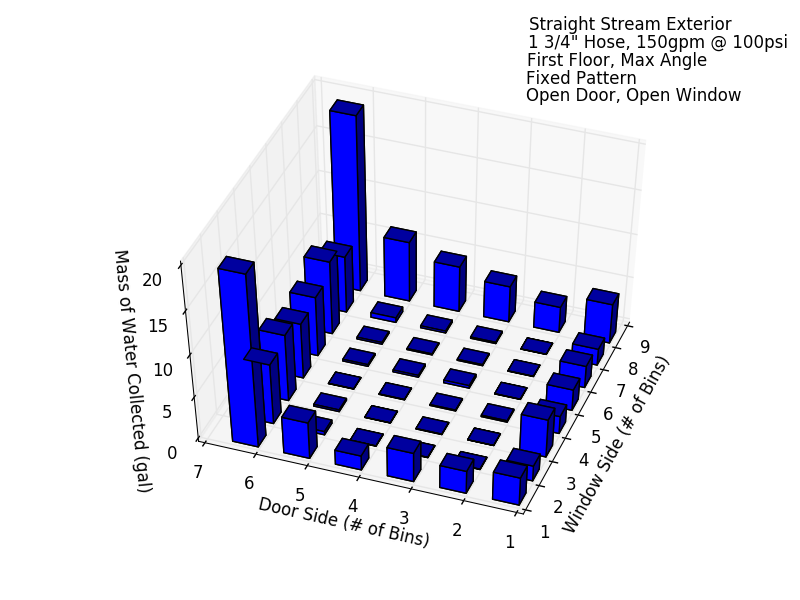
\includegraphics[width=3.2in]{Script_Figures/ADD_Analysis/15-12-10_082039_Datafile_Straight_Stream_Exterior} &
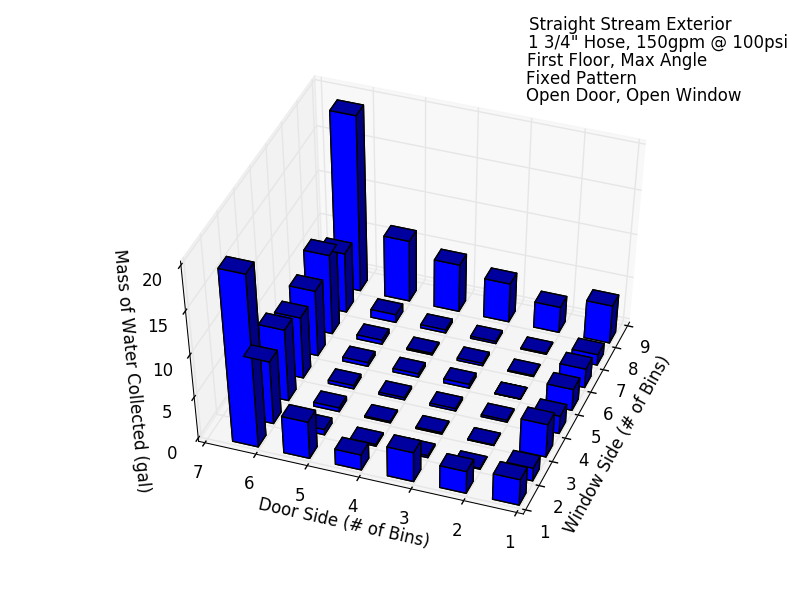
\includegraphics[width=3.2in]{Script_Figures/ADD_Analysis/15-12-10_082423_Datafile_Straight_Stream_Exterior} \\
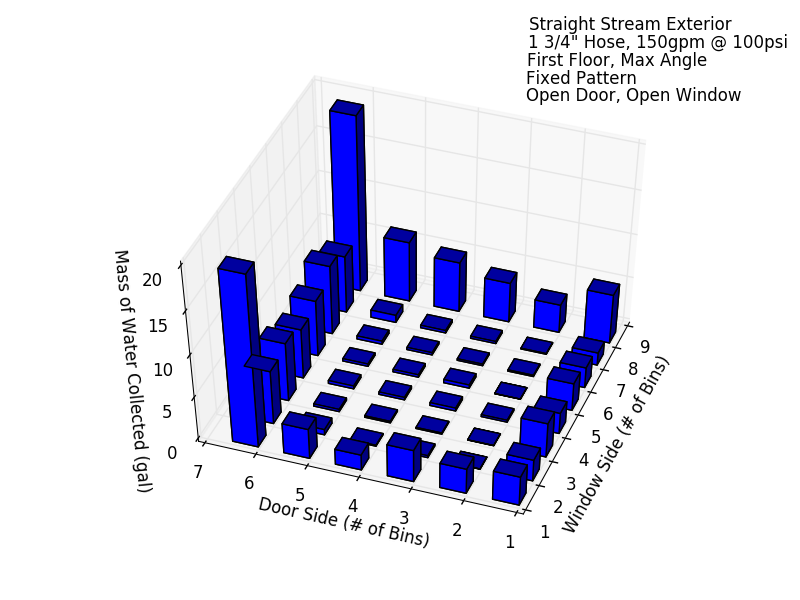
\includegraphics[width=3.2in]{Script_Figures/ADD_Analysis/15-12-10_083305_Datafile_Straight_Stream_Exterior} &
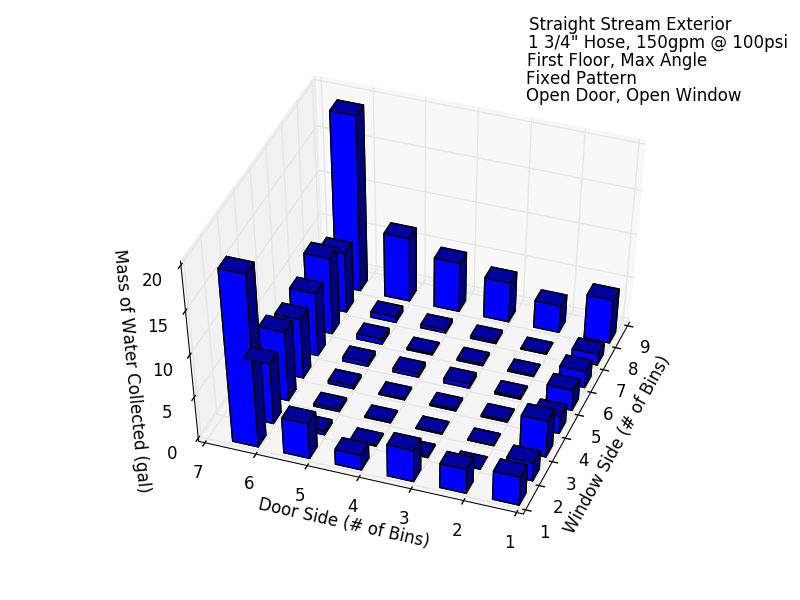
\includegraphics[width=3.2in]{Script_Figures/ADD_Analysis/15-12-10_083751_Datafile_Straight_Stream_Exterior} \\
\end{tabular*}
\caption{Water volume in each collection bin for a fixed exterior straight stream nozzle flowing 150~gpm at 100~psi from the first floor position directed into the structure with a maximum angle. The four bar charts are replicate tests of the same configuration}
\label{fig:Repeatability_Testing}
\end{figure}

Qualitatively, the array of bars in each chart in Figure~\ref{fig:Repeatability_Testing} look similar to one another. However, to better compare the tests, a statistical approach known as an analysis of variance (ANOVA), was performed. Specifically, the Kruskal-Willis one-way ANOVA test was applied. The goal of this analysis was to quantify whether samples (in this case the flow rate of water in each bin) originate from the same distribution (are the tests similar or different). The Kruskal-Willis analysis was selected because there is no prior assumption that the data is normally distributed. While this statistical analysis can compare $n$ number of data sets and identify if the data sets are statistically different, a limitation in all ANOVAs is the inability to identify which data sets are statistically different. The result of the ANOVA is a p-value. If the p-value is less than 0.05, the experiments being compared are statistically different. If the p-value is large, the experiments being compared are not statistically different.

For the straight stream experiments shown in Figure~\ref{fig:Repeatability_Testing}, two Kruskal-Willis ANOVA tests were applied; one was based on average flow rate of water into each collection bin and the other was based on total volume of water recorded in each bin. The resulting p-values were 0.822 and 0.627 for average flow rate and total volume respectively. The high p-values mean that the 4 straight stream flow patterns cannot be distinguished from one another. In other words, these experiments can be considered as repeatable.

Confirmation of repeatability, allowed for the exploration of additional comparisons within the data. The three main comparisons were varying the hose stream type, varying the nozzle direction, and varying the flow pressure. The hose stream comparisons were designed to quantify the impact on water distribution from using a straight stream, smooth bore, or a narrow fog pattern. For the hose stream type comparisons, 6 configurations were analyzed. Within each configuration set, the nozzle direction, nozzle movement, and nozzle pressure/flow rate were fixed. Table~\ref{tab:add_hosestream} shows the results from the ANOVA test based on flow rate and total volume for each of the configurations tested.

\begin{table}[!ht]
\centering
\footnotesize
\caption{Assessment of Variation of Hose Stream Types}
\label{tab:add_hosestream}
\begin{tabular}{lccccc}
\toprule[1.5pt]
Configuration & \# of Tests & P Value Rate & Different & P Value Volume & Different \\ 
\midrule
 Interior, Mid Ceiling, Fixed Pattern             & 3          & 6.6E-07 & \checkmark & 2.3E-05 & \checkmark   \\
 Interior, Mid Ceiling, `O' Pattern               & 3          & 0.008   & \checkmark & 0.008   & \checkmark   \\
 1st Floor Exterior, Max Angle Ceiling, Fixed Pattern  & 3          & 0.046   & \checkmark & 0.100   &    \\
 2nd Floor Exterior, Max Angle Ceiling, Fixed Pattern  & 3          & 0.064   &            & 0.004   & \checkmark   \\
 1st Floor Exterior, Max Angle Ceiling, Sweep Pattern  & 2          & 0.383   &            & 0.337   &    \\
 2nd Floor Exterior, Max Angle Ceiling, Sweep Pattern  & 2          & 0.433   &            & 0.524   &    \\
\bottomrule[1.25pt]
\end{tabular}
\end{table}

The results of the statistical analysis identified that 4 of the 6 hose stream comparisons showed statistical difference in either the flow rate comparison, total volume comparison, or both. In the case of the interior tests, both the fixed pattern and `o' pattern showed statistical differences in both tests (Figures~\ref{fig:Interior_Varying_Nozzle_Types_Fixed_Pattern} and \ref{fig:Interior_Varying_Nozzle_Types_O_Pattern}). Comparison of the three streams in Figure~\ref{fig:Interior_Varying_Nozzle_Types_Fixed_Pattern}, shows that the fog stream had significantly lower volume of water at the edge bins along the wall opposite the doorway. For the interior test with the `o' pattern, the p-test values indicate that the data are different. The volume data in Figure~\ref{fig:Interior_Varying_Nozzle_Types_O_Pattern}, show that patterns along the wall opposite the doorway are similar. The smooth bore had water distributed along the window wall and wall opposite the window compared to the other two hose streams which had the water more concentrated along the wall opposite the doorway; leading to the statistical difference.

\begin{figure}[!ht]
\begin{tabular*}{\textwidth}{lr}
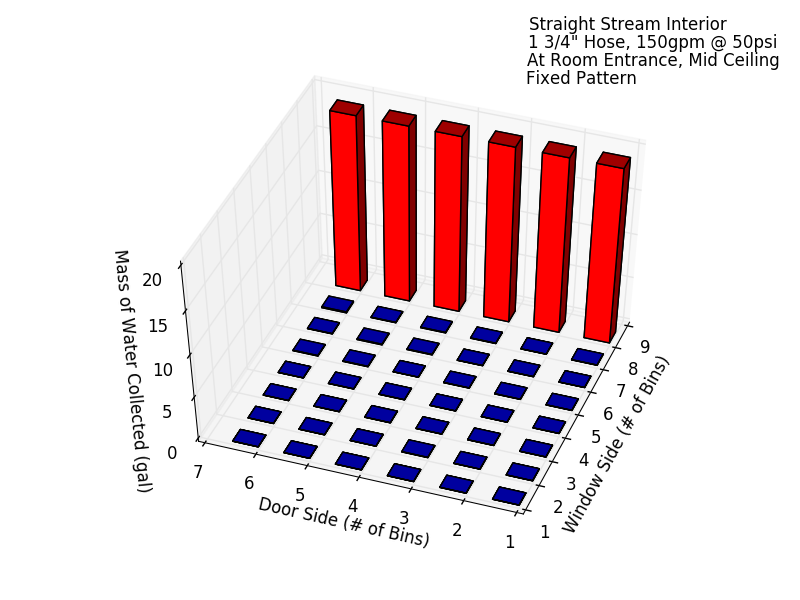
\includegraphics[width=3.2in]{Script_Figures/ADD_Analysis/15-12-09_121955_Datafile_Straight_Stream_Interior} &
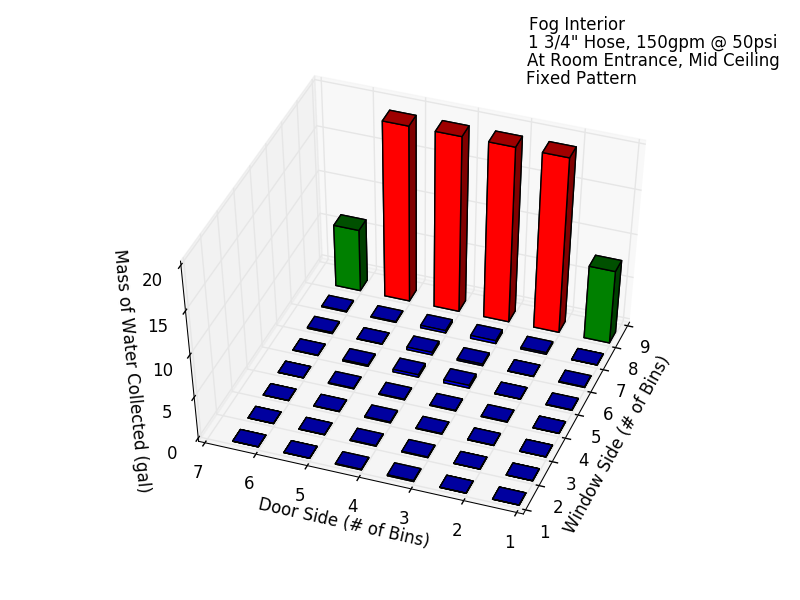
\includegraphics[width=3.2in]{Script_Figures/ADD_Analysis/15-12-09_123142_Datafile_Fog_Interior} \\
\end{tabular*}
\centering
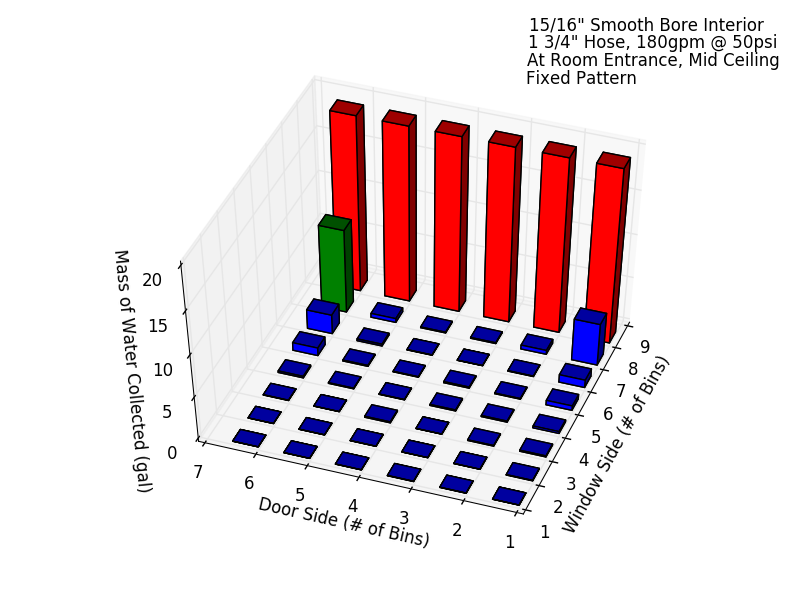
\includegraphics[width=3.2in]{Script_Figures/ADD_Analysis/15-12-09_144839_Datafile_15_16in_Smooth_Bore_Interior}
\caption{Water volume in each collection bin for interior fixed pattern flow at the mid-ceiling direction for a straight stream (upper left), fog (upper right), and smooth bore (bottom middle) nozzle}
\label{fig:Interior_Varying_Nozzle_Types_Fixed_Pattern}
\end{figure}

\begin{figure}[ht]
\begin{tabular*}{\textwidth}{lr}
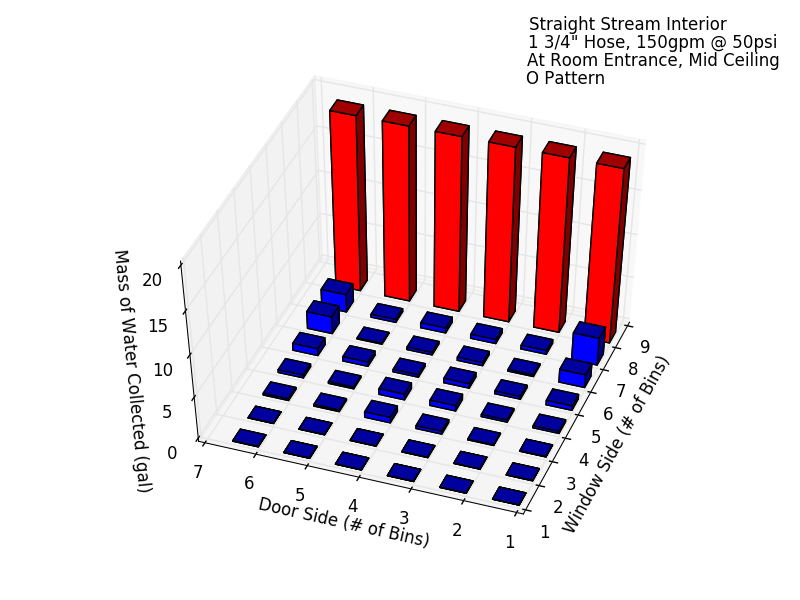
\includegraphics[width=3.2in]{Script_Figures/ADD_Analysis/15-12-09_122551_Datafile_Straight_Stream_Interior} &
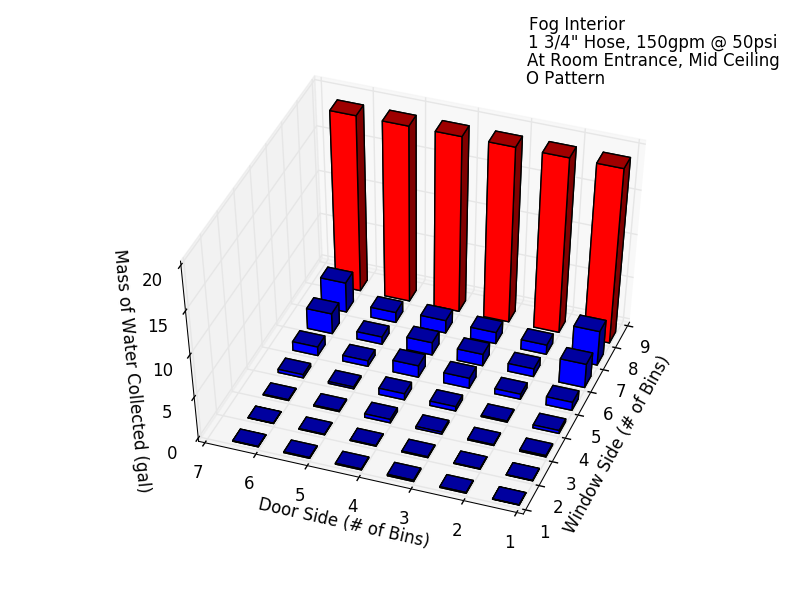
\includegraphics[width=3.2in]{Script_Figures/ADD_Analysis/15-12-09_123636_Datafile_Fog_Interior} \\
\end{tabular*}
\centering
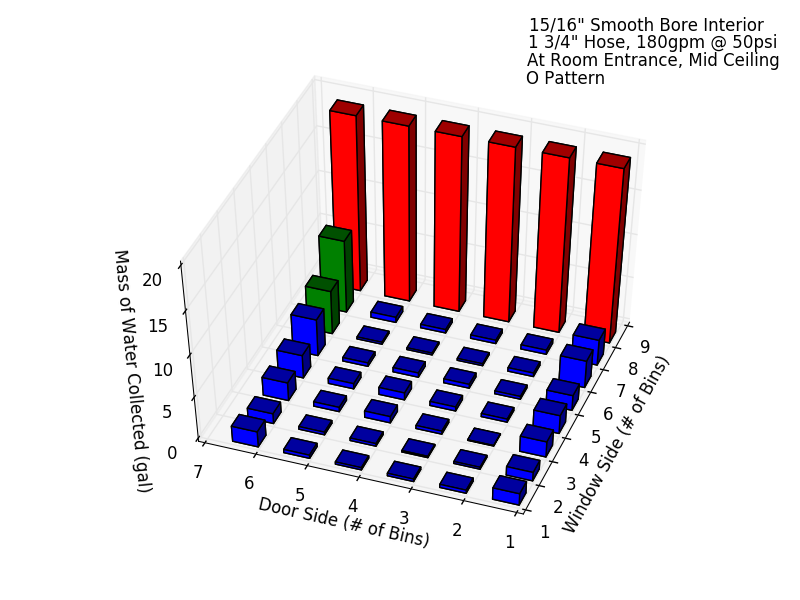
\includegraphics[width=3.2in]{Script_Figures/ADD_Analysis/15-12-09_145534_Datafile_15_16in_Smooth_Bore_Interior}
\caption{Water volume in each collection bin for interior `O' pattern flow at the mid-ceiling direction for a straight stream (upper left), fog (upper right), and smooth bore (bottom middle) nozzle}
\label{fig:Interior_Varying_Nozzle_Types_O_Pattern}
\end{figure}

\clearpage

The statistical tests for the exterior, fixed pattern experiments at the max angle indicated that the first floor tests had a different flow rate distribution and the second floor tests had different total volume distribution. In both the fixed pattern first and second floor tests, the straight stream and smooth bore nozzles showed similar total volume distributions (Figures~\ref{fig:Exterior_FirstFloor_Fixed_Varying_Nozzle} and \ref{fig:Exterior_SecondFloor_Fixed_Varying_Nozzle}). Similar to the interior tests, the fog nozzle shows a different pattern, most noticeably in Figure~\ref{fig:Exterior_SecondFloor_Fixed_Varying_Nozzle}. 

\begin{figure}[ht]
\begin{tabular*}{\textwidth}{lr}
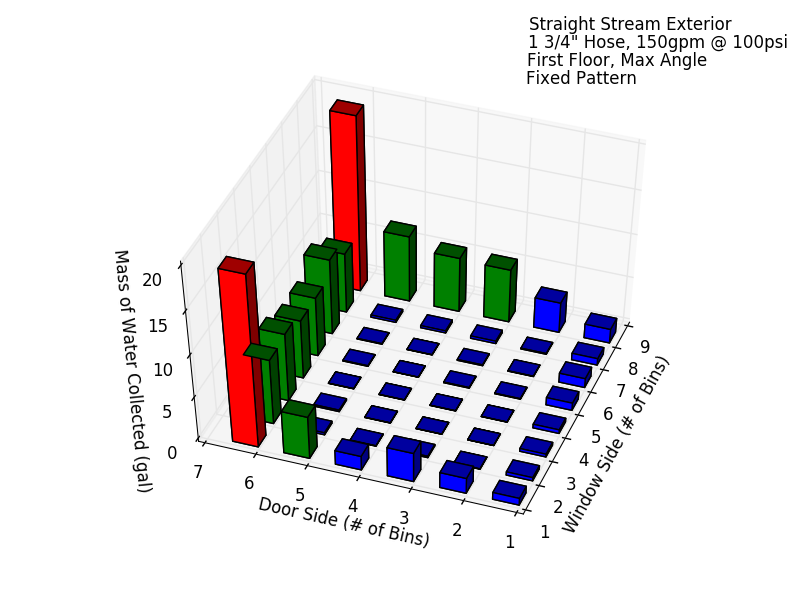
\includegraphics[width=3.2in]{Script_Figures/ADD_Analysis/15-12-08_113237_Datafile_Straight_Stream_Exterior} &
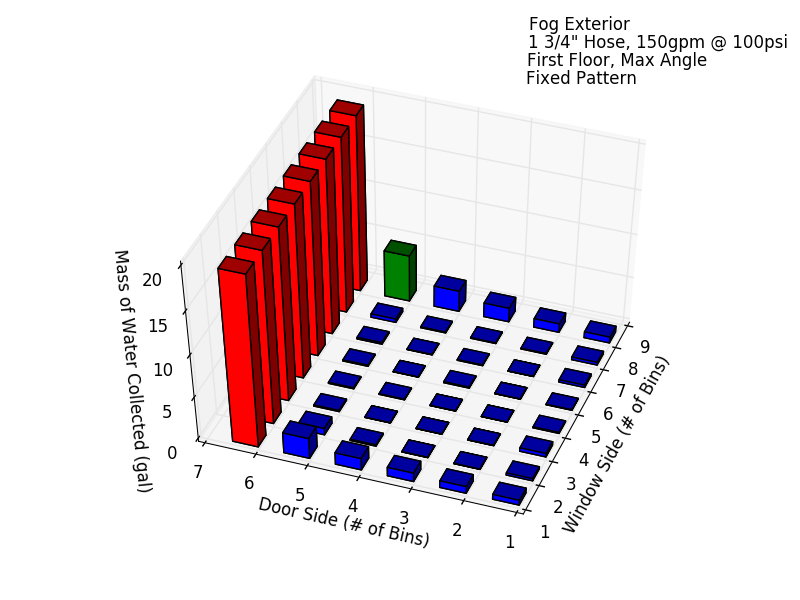
\includegraphics[width=3.2in]{Script_Figures/ADD_Analysis/15-12-08_121806_Datafile_Fog_Exterior} \\
\end{tabular*}
\centering
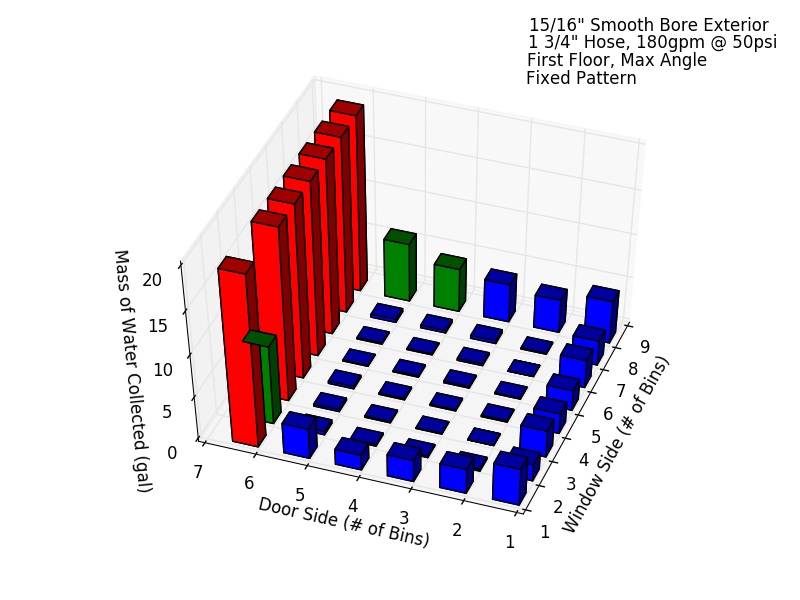
\includegraphics[width=3.2in]{Script_Figures/ADD_Analysis/15-12-08_101028_Datafile_15_16in_Smooth_Bore_Exterior}
\caption{Water volume in each collection bin for exterior first floor fixed pattern flow at the max angle direction for a straight stream (upper left), fog (upper right), and smooth bore (bottom middle) nozzle}
\label{fig:Exterior_FirstFloor_Fixed_Varying_Nozzle}
\end{figure}

\begin{figure}[ht]
\begin{tabular*}{\textwidth}{lr}
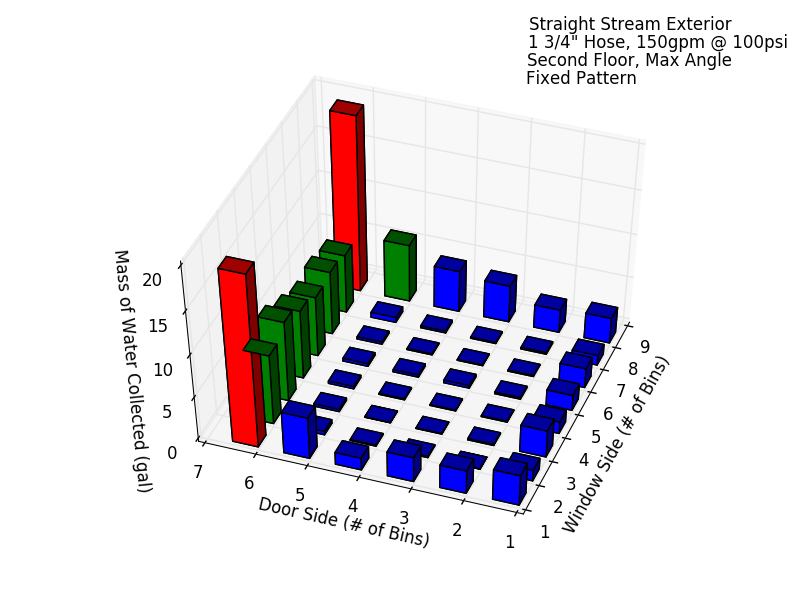
\includegraphics[width=3.2in]{Script_Figures/ADD_Analysis/15-12-07_145156_Datafile_Straight_Stream_Exterior} &
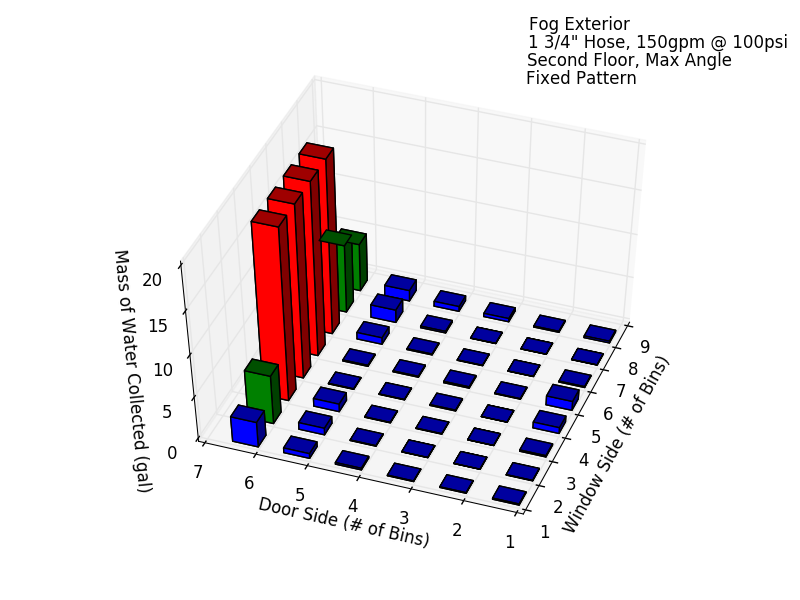
\includegraphics[width=3.2in]{Script_Figures/ADD_Analysis/15-12-07_155751_Datafile_Fog_Exterior} \\
\end{tabular*}
\centering
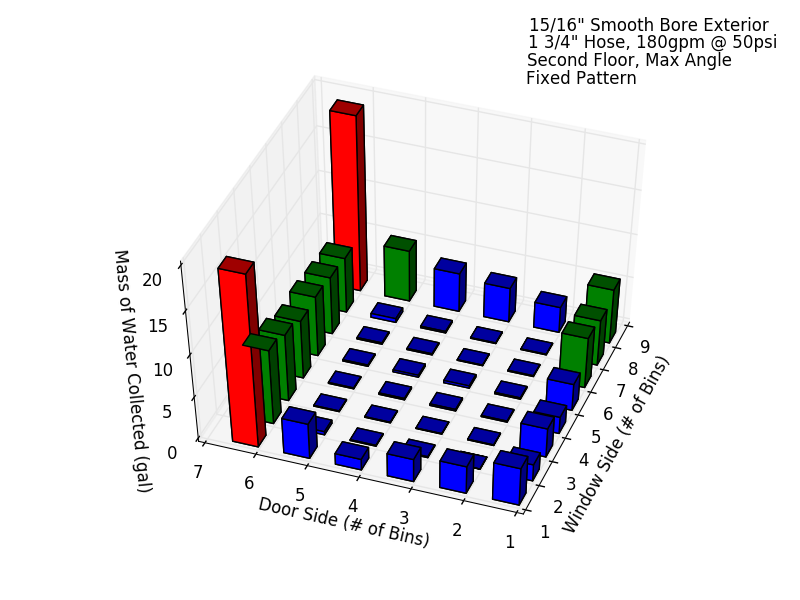
\includegraphics[width=3.2in]{Script_Figures/ADD_Analysis/15-12-07_111118_Datafile_15_16in_Smooth_Bore_Exterior}
\caption{Water volume in each collection bin for exterior second floor fixed pattern flow at the max angle direction for a straight stream (upper left), fog (upper right), and smooth bore (bottom middle) nozzle}
\label{fig:Exterior_SecondFloor_Fixed_Varying_Nozzle}
\end{figure}

\clearpage

Note that for the exterior water flow experiments with a sweep pattern, only a straight stream and smooth bore hose stream are compared. The stream from a fog pattern would typically encompass the ventilation opening, depending on the size of the opening and the distance from the opening. In these experiments, the fog stream enclosed the window, therefore only a fixed pattern was studied. The results from the statistical tests in Table~\ref{tab:add_hosestream}, indicate that the straight stream and smooth bore are likely similar in both rate and volume. Figures~\ref{fig:Exterior_FirstFloor_O_Varying_Nozzle} and \ref{fig:Exterior_SecondFloor_O_Varying_Nozzle} confirm the similarity in the total water distribution.

\begin{figure}[ht]
\begin{tabular*}{\textwidth}{lr}
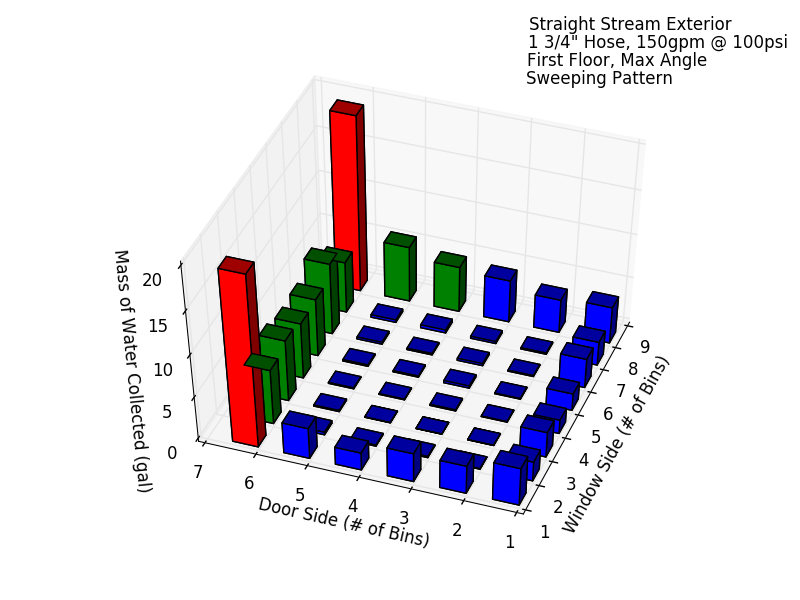
\includegraphics[width=3.2in]{Script_Figures/ADD_Analysis/15-12-08_113716_Datafile_Straight_Stream_Exterior} &
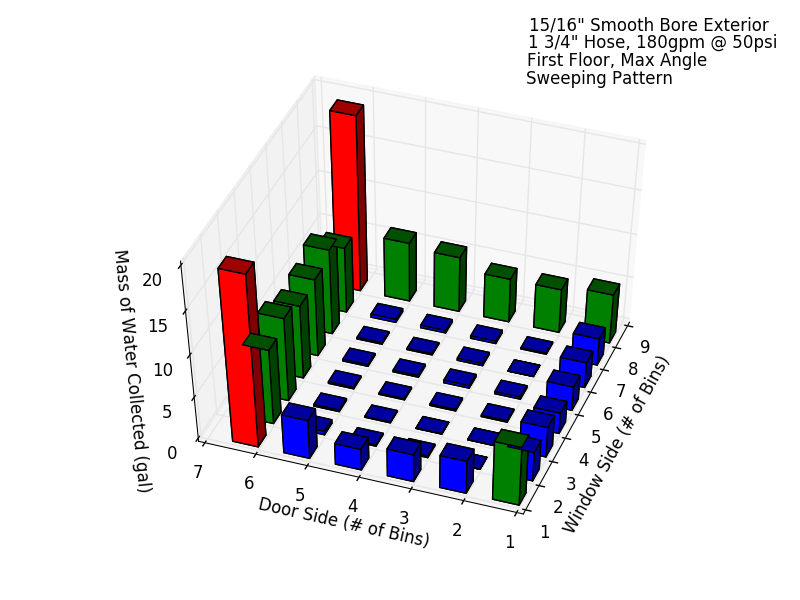
\includegraphics[width=3.2in]{Script_Figures/ADD_Analysis/15-12-08_101825_Datafile_15_16in_Smooth_Bore_Exterior}
\end{tabular*}
\caption{Water volume in each collection bin for exterior first floor sweeping pattern flow at the max angle direction for a straight stream (left) and smooth bore (right) nozzle}
\label{fig:Exterior_FirstFloor_O_Varying_Nozzle}
\end{figure}


\begin{figure}[ht]
\begin{tabular*}{\textwidth}{lr}
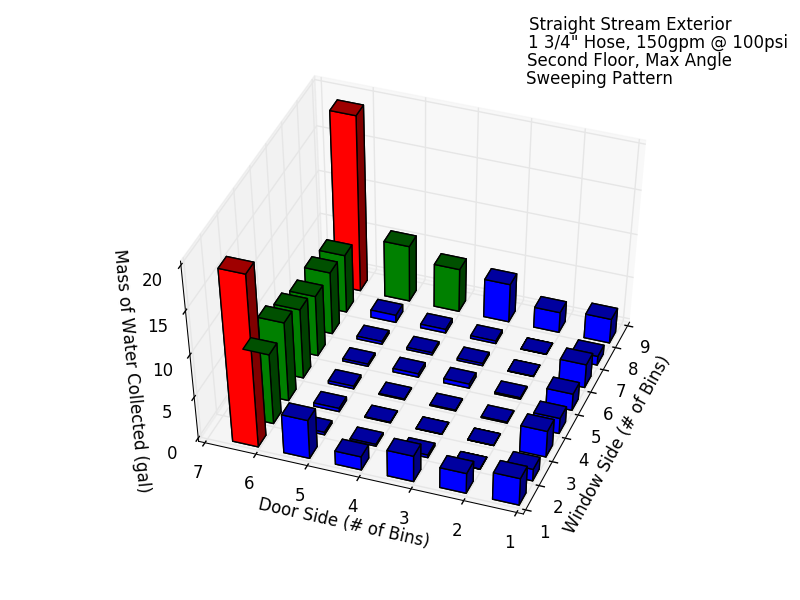
\includegraphics[width=3.2in]{Script_Figures/ADD_Analysis/15-12-07_145842_Datafile_Straight_Stream_Exterior} &
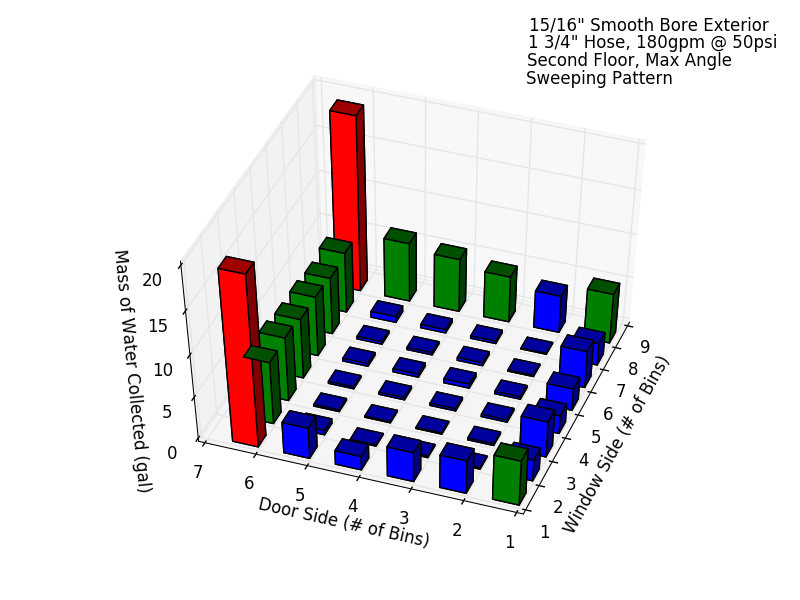
\includegraphics[width=3.2in]{Script_Figures/ADD_Analysis/15-12-07_121014_Datafile_15_16in_Smooth_Bore_Exterior}
\end{tabular*}
\caption{Water volume in each collection bin for exterior second floor sweeping pattern flow at the max angle direction for a straight stream (left) and smooth bore (right) nozzle}
\label{fig:Exterior_SecondFloor_O_Varying_Nozzle}
\end{figure}


\clearpage


The second comparison was to quantify the impact of nozzle direction on water distribution within the compartment. Referring back to Figures~\ref{fig:Nozzle_Direction_Interior_Attack}, \ref{fig:Nozzle_Direction_Exterior_1st_Floor_Attack}, and \ref{fig:Nozzle_Direction_Exterior_2nd_Floor_Attack} there are 3, 5, and 5 nozzle directions for the interior experiments, the exterior first floor experiments, and the exterior second floor experiments, respectively. Table~\ref{tab:add_nozzleposition} shows the p-test values average flow rate per collection bin and total volume per collection bin for the nozzle direction comparison experiments. In all comparisons of nozzle direction, there was enough variation in the flow rate and volume data for the results to be statistically different. For the case where the nozzle direction was the same, but the starting floor (first floor versus second floor) was varied the resulting was distributions was similar.

\begin{table}[!ht]
\centering
\footnotesize
\caption{Assessment of Variation of Nozzle Directions}
\label{tab:add_nozzleposition}
\begin{tabular}{lccccc}
\toprule[1.5pt]
Configuration & \# of Tests & P Value Rate & Different & P Value Volume & Different \\ 
\midrule
 Interior, Smooth Bore, Fixed Pattern                  & 3          & 3.2E-04 & \checkmark & 2.2E-04 & \checkmark   \\
 Interior, Straight Stream, Fixed Pattern              & 3          & 3.0E-09 & \checkmark & 2.0E-08 & \checkmark   \\
 Interior, Smooth Bore, `O' Pattern                    & 3          & 2.0E-04 & \checkmark & 7.8E-05 & \checkmark   \\
 Interior, Straight Stream, `O' Pattern                & 3          & 3.6E-04 & \checkmark & 6.0E-04 & \checkmark   \\
 1st Floor Exterior, Straight Stream, Fixed Pattern    & 5          & 2.8E-08 & \checkmark & 5.6E-08 & \checkmark   \\
 1st Floor Exterior, Smooth Bore Fixed Pattern         & 5          & 1.0E-06 & \checkmark & 3.8E-06 & \checkmark   \\
 2nd Floor Exterior, Straight Stream Fixed Pattern     & 5          & 2.3E-09 & \checkmark & 2.7E-09 & \checkmark   \\
 2nd Floor Exterior, Smooth Bore Fixed Pattern         & 4          & 3.1E-06 & \checkmark & 6.9E-07 & \checkmark   \\
 1st and 2nd Floor, Exterior, Straight Stream          & 2          & 0.143   &            & 0.157   &              \\
\bottomrule[1.25pt]
\end{tabular}
\end{table}

For the interior tests, there were three nozzle directions examined: at wall, mid ceiling, and max angle (Figure~\ref{fig:Nozzle_Direction_Interior_Attack}). The fixed pattern smooth bore and straight stream tests (Figures~\ref{fig:Interior_Varying_Nozzle_Direction_SB_Fixed_Pattern} and \ref{fig:Interior_Varying_Nozzle_Pressure_SS_Fixed_Pattern}) both show variation in the data (Table~\ref{tab:add_nozzleposition}) that is visualized in the total volume bar charts. Specifically, the max angle direction for both hose stream types resulted in spread along the perimeter of the compartment compared to localized water along the wall opposite the doorway. The `o' pattern smooth bore and straight stream tests show are similar to the fixed pattern. The mid ceiling and wall direction show water concentrated along the wall opposite the doorway while the max angle shows water distributed around the perimeter. The ANOVA tests also show that there is statistical difference between the nozzle directions for the moving hose stream at the three directions.

\begin{figure}[ht]
\begin{tabular*}{\textwidth}{lr}
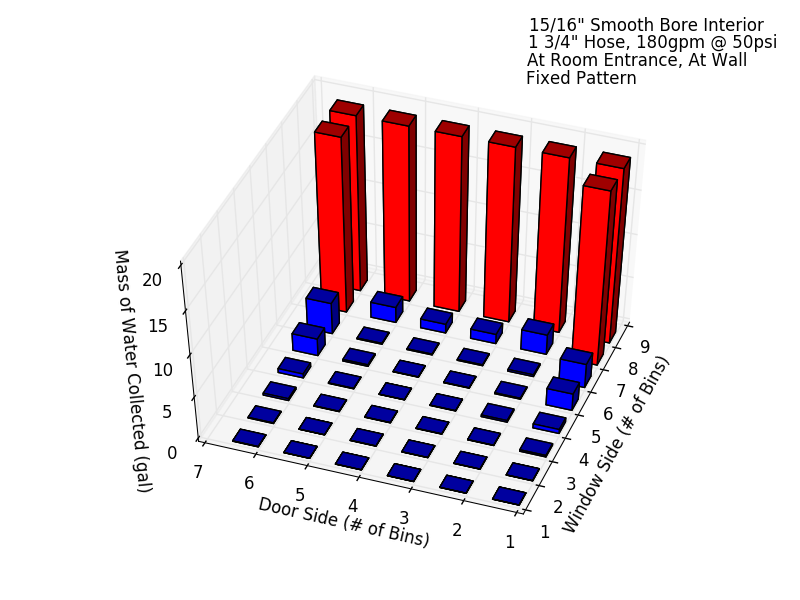
\includegraphics[width=3.2in]{Script_Figures/ADD_Analysis/15-12-09_142948_Datafile_15_16in_Smooth_Bore_Interior} &
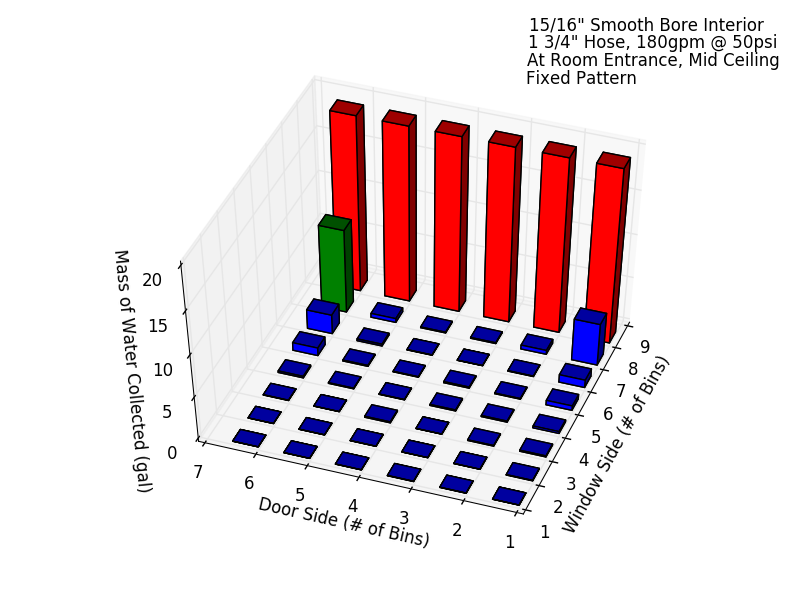
\includegraphics[width=3.2in]{Script_Figures/ADD_Analysis/15-12-09_144839_Datafile_15_16in_Smooth_Bore_Interior} \\
\end{tabular*}
\centering
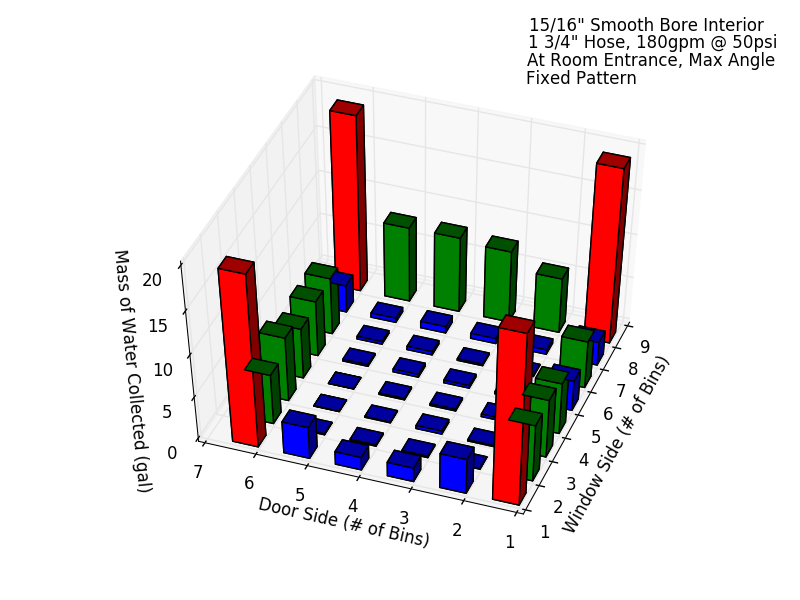
\includegraphics[width=3.2in]{Script_Figures/ADD_Analysis/15-12-09_145932_Datafile_15_16in_Smooth_Bore_Interior}
\caption{Water volume in each collection bin for an interior smooth bore stream with a fixed pattern at three nozzle directions: at wall (top left), mid ceiling (top right) and max angle (bottom)}
\label{fig:Interior_Varying_Nozzle_Direction_SB_Fixed_Pattern}
\end{figure}

\begin{figure}[ht]
\begin{tabular*}{\textwidth}{lr}
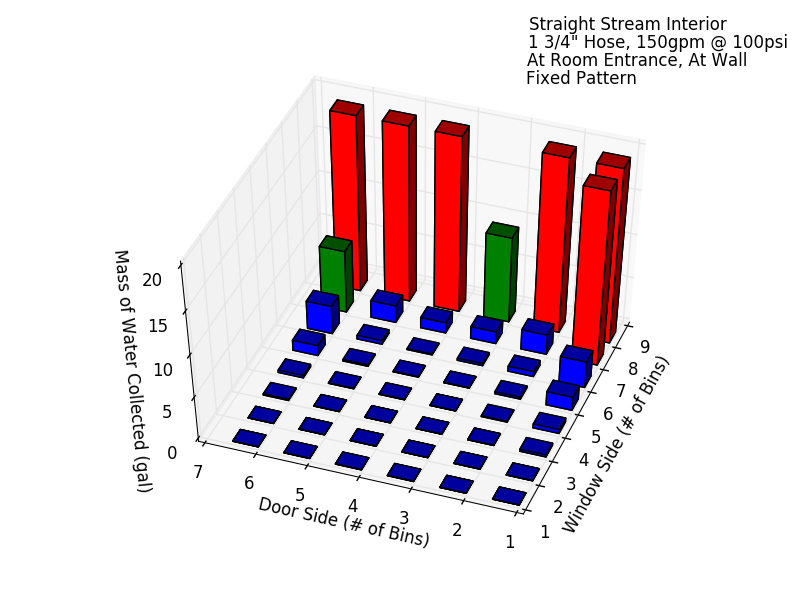
\includegraphics[width=3.2in]{Script_Figures/ADD_Analysis/15-12-09_151401_Datafile_Straight_Stream_Interior} &
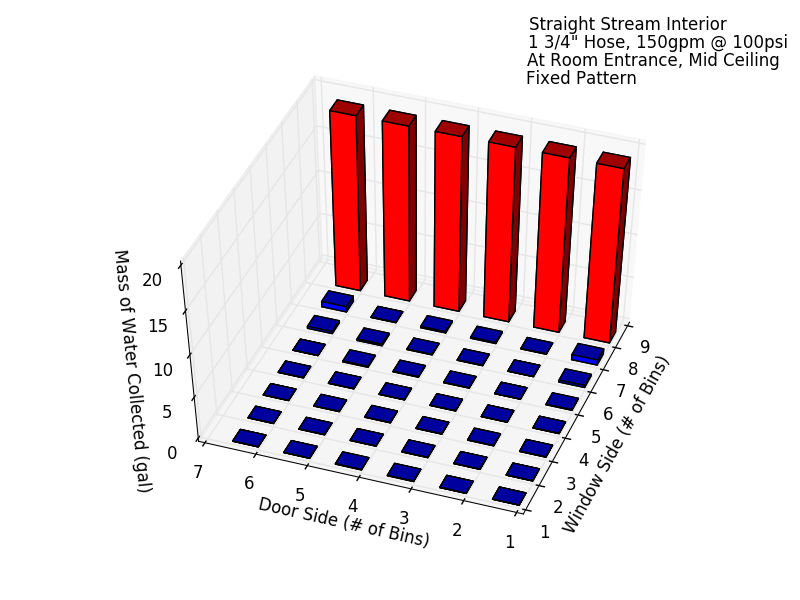
\includegraphics[width=3.2in]{Script_Figures/ADD_Analysis/15-12-09_112850_Datafile_Straight_Stream_Interior} \\
\end{tabular*}
\centering
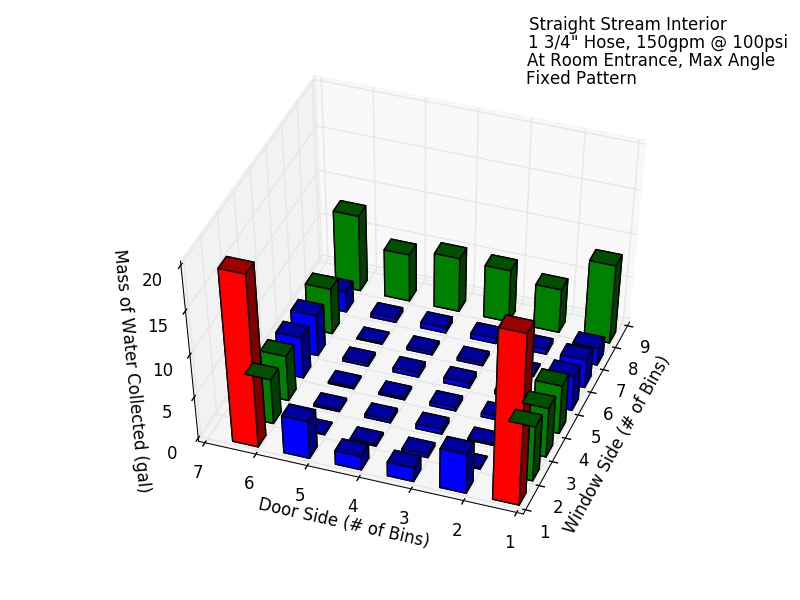
\includegraphics[width=3.2in]{Script_Figures/ADD_Analysis/15-12-09_152435_Datafile_Straight_Stream_Interior}
\caption{Water volume in each collection bin for an interior straight stream with a fixed pattern at three nozzle directions: at wall (top left), mid ceiling (top right) and max angle (bottom)}
\label{fig:Interior_Varying_Nozzle_Direction_SS_Fixed_Pattern}
\end{figure}

\begin{figure}[ht]
\begin{tabular*}{\textwidth}{lr}
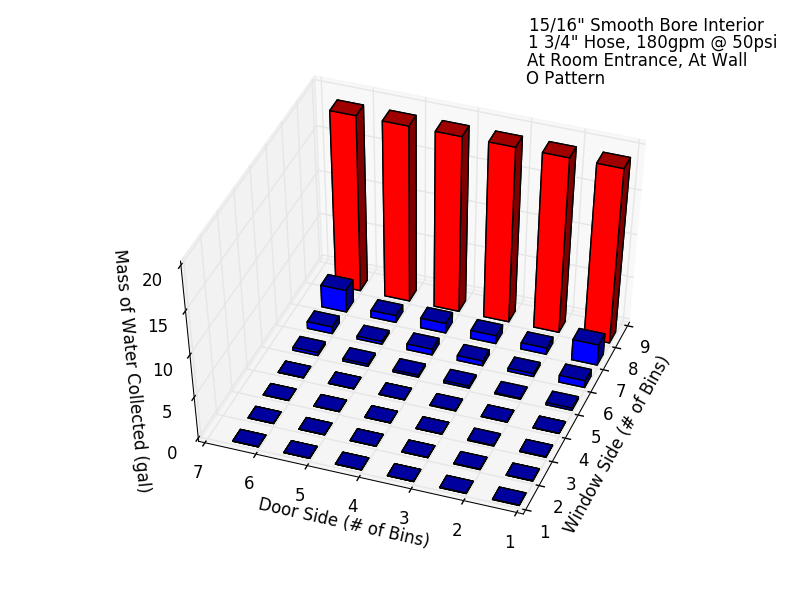
\includegraphics[width=3.2in]{Script_Figures/ADD_Analysis/15-12-09_144524_Datafile_15_16in_Smooth_Bore_Interior} &
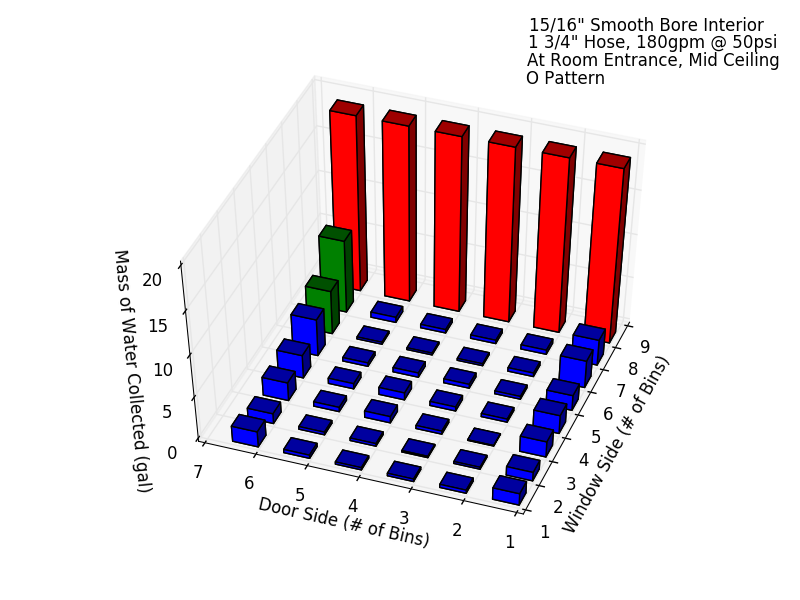
\includegraphics[width=3.2in]{Script_Figures/ADD_Analysis/15-12-09_145534_Datafile_15_16in_Smooth_Bore_Interior} \\
\end{tabular*}
\centering
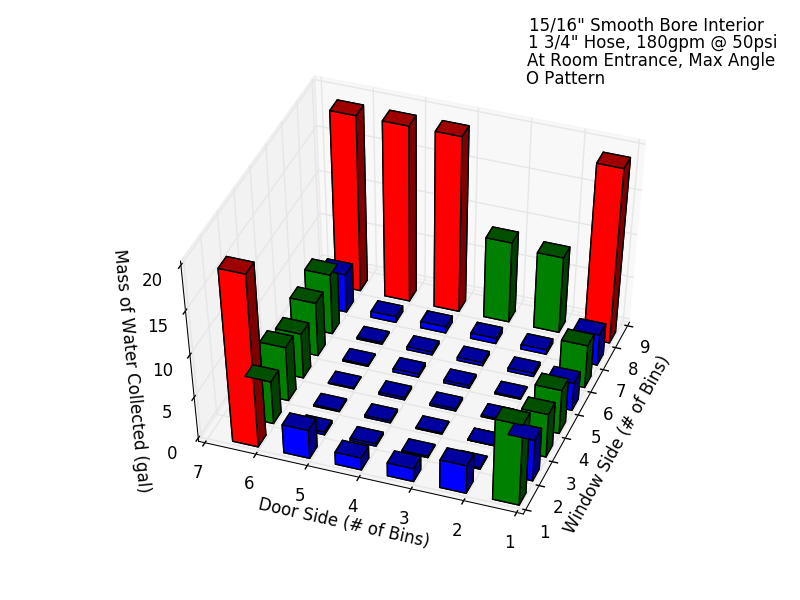
\includegraphics[width=3.2in]{Script_Figures/ADD_Analysis/15-12-09_150300_Datafile_15_16in_Smooth_Bore_Interior}
\caption{FWater volume in each collection bin for an interior smooth bore stream with an `o' pattern at three nozzle directions: at wall (top left), mid ceiling (top right) and max angle (bottom)}
\label{fig:Interior_Varying_Nozzle_Direction_SB_O_Pattern}
\end{figure}

\begin{figure}[ht]
\begin{tabular*}{\textwidth}{lr}
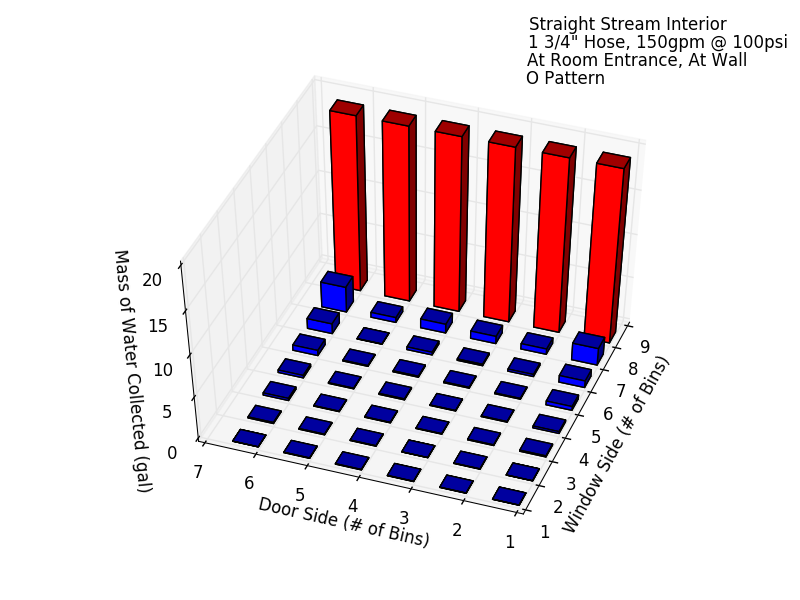
\includegraphics[width=3.2in]{Script_Figures/ADD_Analysis/15-12-09_151823_Datafile_Straight_Stream_Interior} &
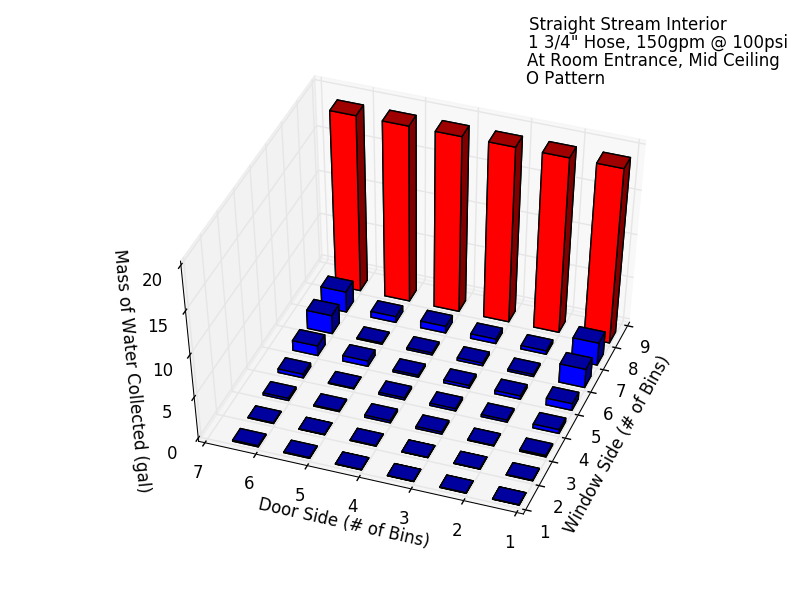
\includegraphics[width=3.2in]{Script_Figures/ADD_Analysis/15-12-09_113335_Datafile_Straight_Stream_Interior} \\
\end{tabular*}
\centering
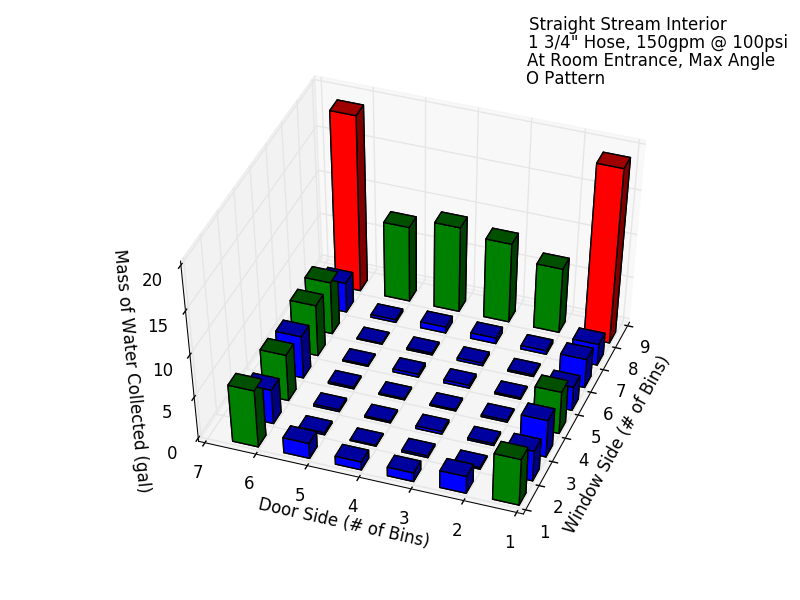
\includegraphics[width=3.2in]{Script_Figures/ADD_Analysis/15-12-09_153038_Datafile_Straight_Stream_Interior}
\caption{Water volume in each collection bin for an interior straight stream with an 'o' pattern at three nozzle directions: at wall (top left), mid ceiling (top right) and max angle (bottom)}
\label{fig:Interior_Varying_Nozzle_Direction_SS_O_Pattern}
\end{figure}

\clearpage

The first floor exterior experiments used 5 different nozzle directions: max angle ceiling, mid ceiling, min angle ceiling, max angle wall, and at wall. The statistical analysis indicated that the 5 nozzle direction results are not the same in terms of flow rate and volume for both the smooth bore and straight stream experiments. Figure~\ref{fig:Exterior_First_Floor_Varying_Nozzle_Directions_SB_Fixed_Pattern} shows the water volume distribution for the 5 directions for the smooth bore stream while Figure~\ref{fig:Exterior_First_Floor_Varying_Nozzle_Directions_SS_Fixed_Pattern} shows the water volume distributions for the straight stream. For both streams, the mid ceiling and min angle ceiling directions indicate that the majority of the water accumulated in the bins along the wall opposite the window. The two wall directions and the max angle ceiling position show a broader distribution of water within in the compartment with the max angle ceiling having the most disperse distribution.

The smooth bore and straight stream second floor exterior experiments were similar to the first floor exterior experiments in that changing nozzle position produced flow rate and volume data that was different as a function of position. Figures~\ref{fig:Exterior_Second_Floor_Varying_Nozzle_Directions_SB_Fixed_Pattern} and \ref{fig:Exterior_Second_Floor_Varying_Nozzle_Directions_SS_Fixed_Pattern} show the results of the water volume distribution for 4 smooth bore directions and 5 straight stream directions. Like all of the prior position data presented, the max angle ceiling shows the most prominent water distribution with water filling the compartment perimeter buckets, noticeably different than the other wall or ceiling directions. The one exception here is the straight stream soffit experiment shows a flatter overall distribution. 

\begin{figure}[ht]
\begin{tabular*}{\textwidth}{lr}
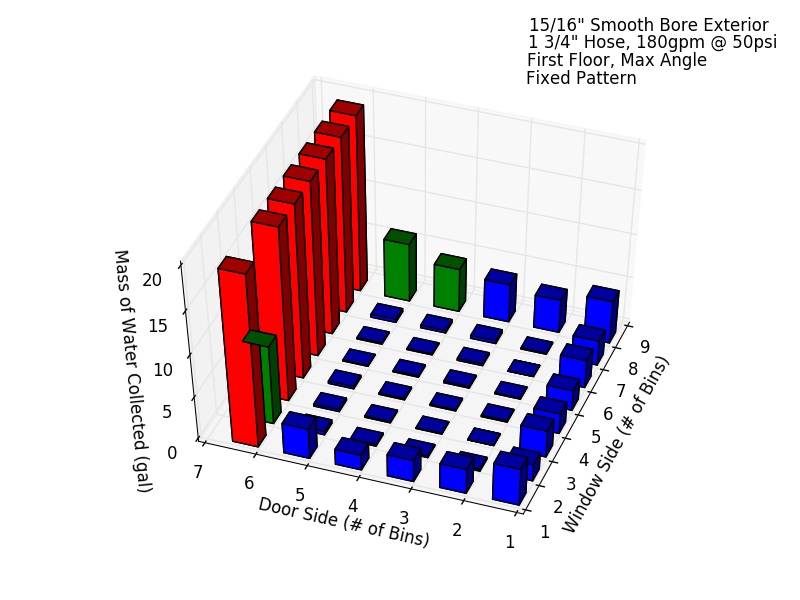
\includegraphics[width=3.2in]{Script_Figures/ADD_Analysis/15-12-08_101028_Datafile_15_16in_Smooth_Bore_Exterior} &
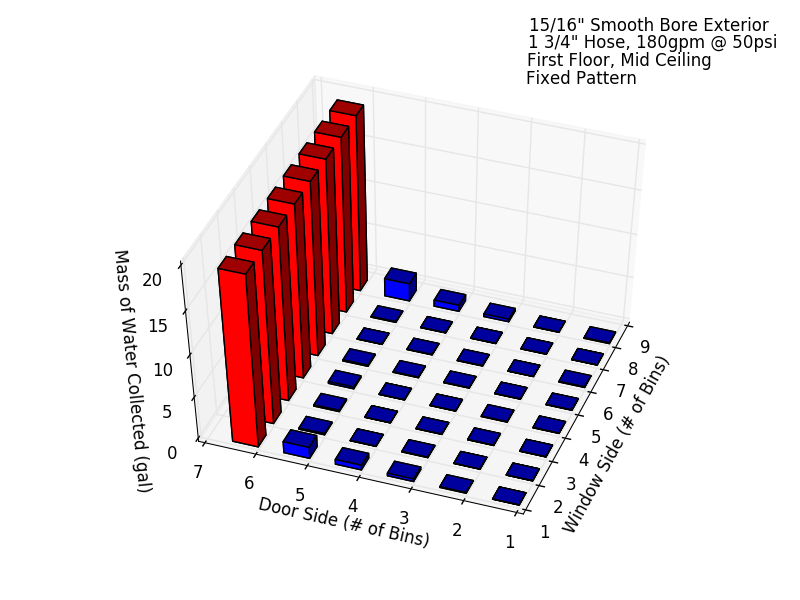
\includegraphics[width=3.2in]{Script_Figures/ADD_Analysis/15-12-08_102802_Datafile_15_16in_Smooth_Bore_Exterior} \\
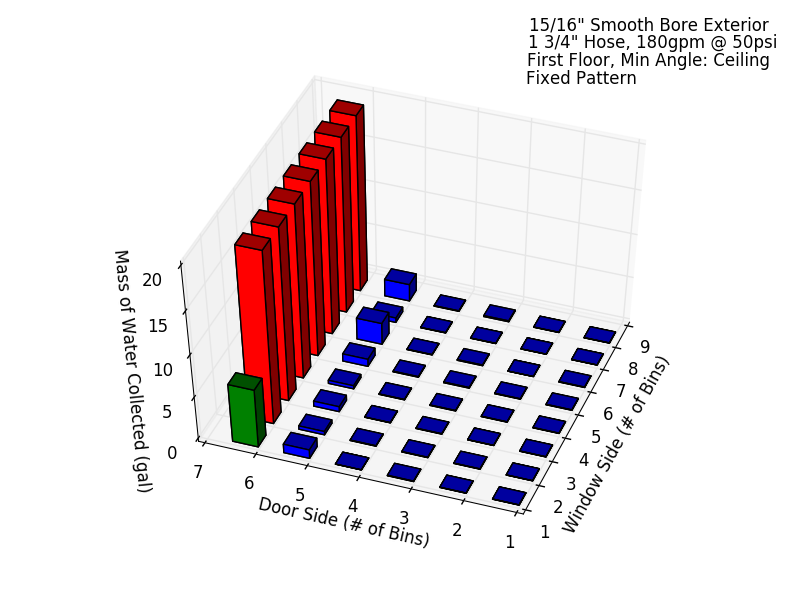
\includegraphics[width=3.2in]{Script_Figures/ADD_Analysis/15-12-08_103414_Datafile_15_16in_Smooth_Bore_Exterior} &
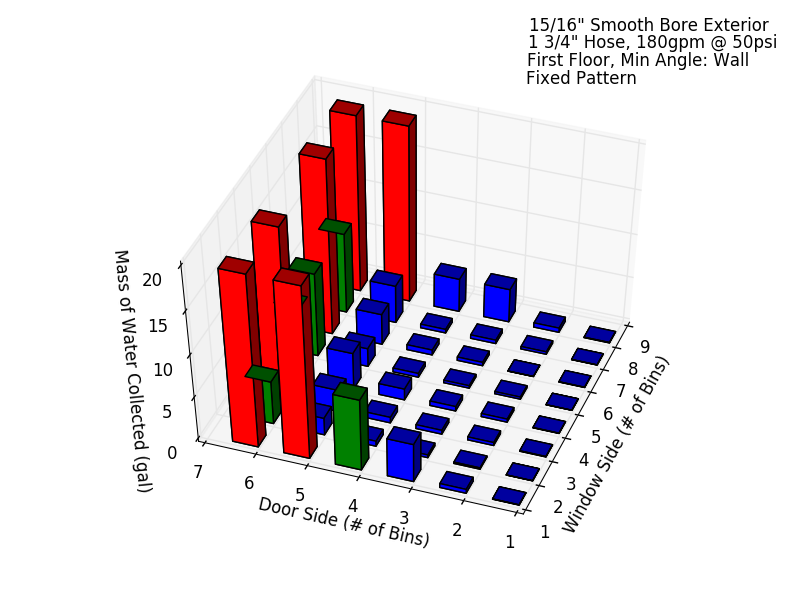
\includegraphics[width=3.2in]{Script_Figures/ADD_Analysis/15-12-08_104150_Datafile_15_16in_Smooth_Bore_Exterior} \\
\end{tabular*}
\centering
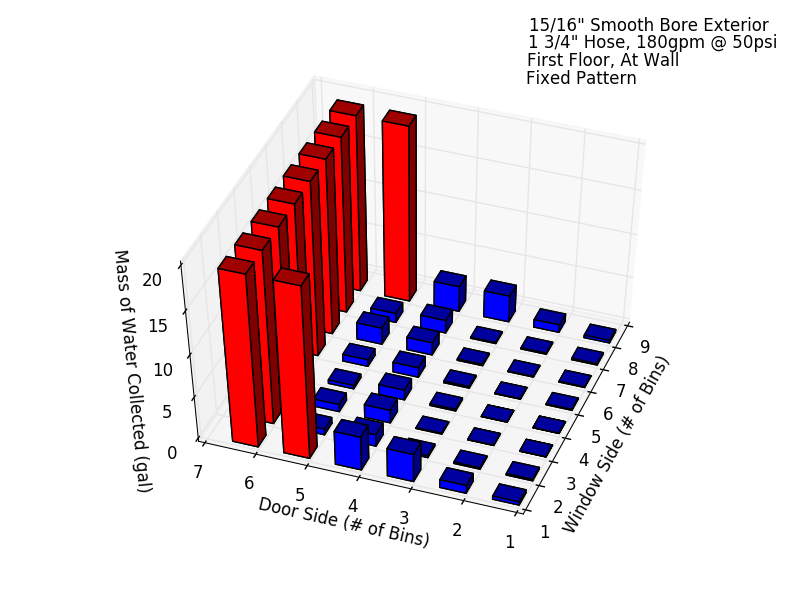
\includegraphics[width=3.2in]{Script_Figures/ADD_Analysis/15-12-08_104620_Datafile_15_16in_Smooth_Bore_Exterior} \\
\caption{Water volume in each collection bin for a first floor exterior smooth bore stream with a fixed pattern at five nozzle directions: max angle (top left), mid ceiling (top right), min angle ceiling (middle left), min angle at wall (middle right), and at wall (bottom)}
\label{fig:Exterior_First_Floor_Varying_Nozzle_Directions_SB_Fixed_Pattern}
\end{figure}

\begin{figure}[ht]
\begin{tabular*}{\textwidth}{lr}
\includegraphics[width=3.2in]{Script_Figures/ADD_Analysis/15-12-08_113237_Datafile_Straight_Stream_Exterior} &
\includegraphics[width=3.2in]{Script_Figures/ADD_Analysis/15-12-08_114905_Datafile_Straight_Stream_Exterior} \\
\includegraphics[width=3.2in]{Script_Figures/ADD_Analysis/15-12-08_120311_Datafile_Straight_Stream_Exterior} &
\includegraphics[width=3.2in]{Script_Figures/ADD_Analysis/15-12-08_121011_Datafile_Straight_Stream_Exterior} \\
\end{tabular*}
\centering
\includegraphics[width=3.2in]{Script_Figures/ADD_Analysis/15-12-08_121425_Datafile_Straight_Stream_Exterior} \\
\caption{Water volume in each collection bin for a first floor exterior straight stream with a fixed pattern at five nozzle directions: max angle (top left), mid ceiling (top right), min angle ceiling (middle left), min angle at wall (middle right), and at wall (bottom)}
\label{fig:Exterior_First_Floor_Varying_Nozzle_Directions_SS_Fixed_Pattern}
\end{figure}

\begin{figure}[ht]
\begin{tabular*}{\textwidth}{lr}
\includegraphics[width=3.2in]{Script_Figures/ADD_Analysis/15-12-07_111118_Datafile_15_16in_Smooth_Bore_Exterior} &
\includegraphics[width=3.2in]{Script_Figures/ADD_Analysis/15-12-07_122135_Datafile_15_16in_Smooth_Bore_Exterior} \\
\includegraphics[width=3.2in]{Script_Figures/ADD_Analysis/15-12-07_140034_Datafile_15_16in_Smooth_Bore_Exterior} &
\includegraphics[width=3.2in]{Script_Figures/ADD_Analysis/15-12-07_141333_Datafile_15_16in_Smooth_Bore_Exterior} \\
\end{tabular*}
\caption{Water volume in each collection bin for a second floor exterior smooth bore stream with a fixed pattern at four nozzle directions: max angle (top left), mid ceiling (top right), min angle ceiling (bottom left), and min angle wall (bottom left)}
\label{fig:Exterior_Second_Floor_Varying_Nozzle_Directions_SB_Fixed_Pattern}
\end{figure}

\begin{figure}[ht]
\begin{tabular*}{\textwidth}{lr}
\includegraphics[width=3.2in]{Script_Figures/ADD_Analysis/15-12-07_145156_Datafile_Straight_Stream_Exterior} &
\includegraphics[width=3.2in]{Script_Figures/ADD_Analysis/15-12-07_151001_Datafile_Straight_Stream_Exterior} \\
\includegraphics[width=3.2in]{Script_Figures/ADD_Analysis/15-12-07_151630_Datafile_Straight_Stream_Exterior} &
\includegraphics[width=3.2in]{Script_Figures/ADD_Analysis/15-12-07_152028_Datafile_Straight_Stream_Exterior} \\
\end{tabular*}
\centering
\includegraphics[width=3.2in]{Script_Figures/ADD_Analysis/15-12-07_155226_Datafile_Straight_Stream_Exterior} \\
\caption{Water volume in each collection bin for a second floor exterior straight stream with a fixed pattern at five nozzle directions: max angle (top left), max angle still (top right), mid ceiling (middle left), min angle ceiling (middle right), and min angle wall (bottom)}
\label{fig:Exterior_Second_Floor_Varying_Nozzle_Directions_SS_Fixed_Pattern}
\end{figure}

\clearpage

For the comparison of a first floor exterior stream to a second floor exterior stream, both with the max angle ceiling nozzle direction the stochastic test showed that the water distributions cannot be distinguished. Figure~\ref{fig:Exterior_First_Floor_Second_Floor} shows the volume distribution of water for both cases which can be used to qualitatively confirm the similarity.

\begin{figure}[ht]
\includegraphics[width=3.2in]{Script_Figures/ADD_Analysis/15-12-08_113237_Datafile_Straight_Stream_Exterior}
\includegraphics[width=3.2in]{Script_Figures/ADD_Analysis/15-12-07_145156_Datafile_Straight_Stream_Exterior} \\ 
\caption{Water volume in each collection bin for a first floor exterior straight stream at max angle ceiling (left) and a second floor exterior straight stream at max angle ceiling(right)}
\label{fig:Exterior_First_Floor_Second_Floor}
\end{figure}

\clearpage

The third analysis was to quantify the impact of pressure and flow rate on water distribution within the compartment. Table~\ref{tab:add_pressure} shows the statistical comparison results for the rate of water accumulation and total water volume distribution. Three comparisons examined the impact of changing pressure on a straight stream (Fig.~\ref{fig:Interior_Varying_Nozzle_Pressure_SS_Fixed_Pattern}), changing pressure on a fog stream (Fig.~\ref{fig:Interior_Varying_Nozzle_Pressure_Fog_Fixed_Pattern}) and on a smooth bore stream (Fig.~\ref{fig:Exterior_First_Floor_Varying_Nozzle_Pressure_SB_Fixed_Pattern}). For each of the three hose streams, the statistical analysis of the distributions of flow rate revealed that the distributions could not be distinguished from one another. The p-values based on the volume distributions for the straight stream and fog stream showed statistical differences. However, a qualitative examination of the volume distributions in Figs.~\ref{fig:Interior_Varying_Nozzle_Pressure_SS_Fixed_Pattern} and \ref{fig:Interior_Varying_Nozzle_Pressure_Fog_Fixed_Pattern} shows the similar patterns as a function of pressure for the straight stream and smooth bore hose streams. The majority of the water accumulated along the wall opposite the doorway.

\begin{table}[!ht]
\centering
\footnotesize
\caption{Assessment of Variation of Nozzle Pressure/Flowrate}
\label{tab:add_pressure}
\begin{tabular}{lccccc}
\toprule[1.5pt]
Configuration & \# of Tests & P Value Rate & Different & P Value Volume & Different \\ 
\midrule
 Interior, Straight Stream, Mid Ceiling                  & 3   & 0.277   &            & 0.031   & \checkmark   \\
 Interior, Fog Stream, Mid Ceiling                       & 3   & 0.198   &            & 0.028   & \checkmark   \\
 1st Floor Exterior, Smooth Bore, Max Angle Ceiling      & 3   & 0.750   &            & 0.451   &    \\
 1st Floor Exterior Smooth Bore, Vary Tip Size           & 3   & 0.205   &            & 0.166   &    \\
 1st Floor Exterior, Straight Stream, Max Angle Ceiling  & 2   & 0.971   &            & 0.134   &    \\
 1st Floor Exterior, Varying Stream, Varying Hose Diameter & 2 & 0.491   &            & 0.883   &    \\
 1st Floor Exterior, Smooth Bore, Varying Bail           & 2   & 9.2E-4  & \checkmark & 0.026   & \checkmark   \\

\bottomrule[1.25pt]
\end{tabular}
\end{table}

\begin{figure}[ht]
\begin{tabular*}{\textwidth}{lr}
\includegraphics[width=3.2in]{Script_Figures/ADD_Analysis/15-12-09_112850_Datafile_Straight_Stream_Interior} &
\includegraphics[width=3.2in]{Script_Figures/ADD_Analysis/15-12-09_115707_Datafile_Straight_Stream_Interior} \\
\end{tabular*}
\centering
\includegraphics[width=3.2in]{Script_Figures/ADD_Analysis/15-12-09_121955_Datafile_Straight_Stream_Interior}
\caption{Water volume in each collection bin for an interior straight stream with a fixed pattern at 150~gpm with 100~psi (top left), 75~psi (top right) and 50~psi (bottom)}
\label{fig:Interior_Varying_Nozzle_Pressure_SS_Fixed_Pattern}
\end{figure}

\begin{figure}[ht]
\begin{tabular*}{\textwidth}{lr}
\includegraphics[width=3.2in]{Script_Figures/ADD_Analysis/15-12-09_113802_Datafile_Fog_Interior} &
\includegraphics[width=3.2in]{Script_Figures/ADD_Analysis/15-12-09_120821_Datafile_Fog_Interior} \\
\end{tabular*}
\centering
\includegraphics[width=3.2in]{Script_Figures/ADD_Analysis/15-12-09_123142_Datafile_Fog_Interior}
\caption{Water volume in each collection bin for an interior fog stream with a fixed pattern at 150~gpm with 100~psi (top left), 75~psi (top right) and 50~psi (bottom)}
\label{fig:Interior_Varying_Nozzle_Pressure_Fog_Fixed_Pattern}
\end{figure}

\begin{figure}[ht]
\begin{tabular*}{\textwidth}{lr}
\includegraphics[width=3.2in]{Script_Figures/ADD_Analysis/15-12-08_101028_Datafile_15_16in_Smooth_Bore_Exterior} &
\includegraphics[width=3.2in]{Script_Figures/ADD_Analysis/15-12-08_154306_Datafile_15_16in_Smooth_Bore_Exterior} \\
\end{tabular*}
\centering
\includegraphics[width=3.2in]{Script_Figures/ADD_Analysis/15-12-08_154812_Datafile_15_16in_Smooth_Bore_Exterior}
\caption{Water volume in each collection bin for a first floor exterior smooth bore a fixed pattern with 180~gpm at 50~psi (top left), 150~gpm at 30~psi (top right) and 130~gpm at 15~psi (bottom)}
\label{fig:Exterior_First_Floor_Varying_Nozzle_Pressure_SB_Fixed_Pattern}
\end{figure}

\clearpage

\begin{figure}[ht]
\begin{tabular*}{\textwidth}{lr}
\includegraphics[width=3.2in]{Script_Figures/ADD_Analysis/15-12-07_111118_Datafile_15_16in_Smooth_Bore_Exterior} &
\includegraphics[width=3.2in]{Script_Figures/ADD_Analysis/15-12-07_143141_Datafile__7_8in_Smooth_Bore_Exterior} \\
\end{tabular*}
\centering
\includegraphics[width=3.2in]{Script_Figures/ADD_Analysis/15-12-07_143828_Datafile_1in_Smooth_Bore_Exterior}
\caption{Water volume in each collection bin for an exterior smooth bore stream with a fixed pattern with a 15/16~in. tip (top left), 7/8~in. tip (top right) and 1~in. tip (bottom)}
\label{fig:Exterior_Second_Floor_Varying_Flow_Rates_SB_Fixed_Pattern}
\end{figure}

\begin{figure}[ht]
\includegraphics[width=3.2in]{Script_Figures/ADD_Analysis/15-12-08_162126_Datafile_Straight_Stream_Exterior}
\includegraphics[width=3.2in]{Script_Figures/ADD_Analysis/15-12-08_160630_Datafile_Straight_Stream_Exterior} \\ 
\caption{Water volume in each collection bin for a first floor exterior straight stream with a fixed pattern at 50~psi with 185~gpm (left) and 150~gpm (right)}
\label{fig:Exterior_First_Floor_Varying_Nozzle_Pressure_SS_Fixed_Pattern}
\end{figure}

\begin{figure}[ht]
\includegraphics[width=3.2in]{Script_Figures/ADD_Analysis/15-12-08_140501_Datafile_Straight_Stream_Exterior}
\includegraphics[width=3.2in]{Script_Figures/ADD_Analysis/15-12-08_144238_Datafile_1_1_4in_Smooth_Bore_Exterior} \\ 
\caption{Water volume in each collection bin for a first floor exterior stream with a fixed pattern from 1 3/4~in straight stream (left) and 2 1/2 in smooth bore with 1 1/4 in tip (right)}
\label{fig:Exterior_First_Floor_Varying_Hose_Size}
\end{figure}

\begin{figure}[ht]
\includegraphics[width=3.2in]{Script_Figures/ADD_Analysis/15-12-08_103414_Datafile_15_16in_Smooth_Bore_Exterior}
\includegraphics[width=3.2in]{Script_Figures/ADD_Analysis/15-12-08_153737_Datafile_15_16in_Smooth_Bore_Exterior} \\ 
\caption{Water volume in each collection bin for a first floor exterior smooth bore with a fixed pattern from full open bail (left) and a 1/2 open bail (right)}
\label{fig:Exterior_First_Floor_Varying_Bail}
\end{figure}



\section{Future Research Needs}

The water distribution data presented in this report is a one piece of the fire attack study. The intention of this report is to provide preliminary results and insight into the distribution of water within a compartment. The air entrainment data and full-scale fire testing data are currently undergoing analysis. Upon completion of the analysis, conclusions can be drawn and tactical considerations can be developed regarding each experimental series, the relationships between the series, and the project in its entirety.  

\section{Summary}

The goal of the experiments was quantify water distributions within a room over a set of parameters typical the the fire service. 

% \vspace*{\baselineskip}
% \noindent \bf{Air Entrainment} -
% \normalfont
% \begin{itemize}
% 	\item Air entrainment is dependent on hose stream type. (smooth bore, straight stream, fog)
% 	\item Air entrainment is dependent on structure size, compartmentalization, and ventilation configurations.
% 	\item Increases in nozzle movement increase overall air entrainment.
% 	\item Different nozzle movement patterns have little effect on overall air entrainment. (O, T, Z, inverted U)
% 	\item Air entrainment, either into or out of the structure, is dependent on the horizontal distance of the nozzle to the ventilation opening.
% 	\end{itemize}
% \vspace*{\baselineskip}
% \noindent \bf{Water Distribution} -
% \normalfont
% \begin{itemize}
% 	\item Water distribution is dependent on hose stream type. (smooth bore, straight stream, fog)
% 	\item Water distribution is dependent on stream elevation angle within a compartment.
% 	\item Varying water pressure at the nozzle and flow rate can affect the total amount of water applied to a given area; however, the distribution location can remain constant.
% 	\item Deflecting the hose stream off the ceiling or opposite wall of a compartment can coat the surfaces while applying little water to the center of the room.
% 	\end{itemize}
% \vspace*{\baselineskip}

% \bibliography{UL_general,FireAttackReport}

\clearpage

\appendix

% \section{Air Entrainment Figures}
% \label{app:Air_Entrainment_Figures}

% \subsection{Manufacturer Comparison}

% \begin{figure}[!ht]
% \begin{tabular*}{\textwidth}{lr}
% \includegraphics[width=3.5in]{Script_Figures/Entrainment/Manufacturer_1_5_Combination_Nozzle_95gpm_100psi} &
% \includegraphics[width=3.5in]{Script_Figures/Entrainment/Manufacturer_1_5_Combination_Nozzle_150gpm_50psi} \\
% \includegraphics[width=3.5in]{Script_Figures/Entrainment/Manufacturer_1_5_Combination_Nozzle_150gpm_75psi} &
% \includegraphics[width=3.5in]{Script_Figures/Entrainment/Manufacturer_1_5_Combination_Nozzle_150gpm_100psi} \\
% \end{tabular*}
% \caption{Figures showing manufacturer comparison of interior air entrainment results for 1.5 in combination nozzles.}
% \label{fig:1_5_Interior_Combination_Manufacturer}
% \end{figure}

% \clearpage

% \begin{figure}[!ht]
% \begin{tabular*}{\textwidth}{lr}
% \includegraphics[width=3.5in]{Script_Figures/Entrainment/Manufacturer_1_5_Smooth_Bore_Nozzle_7_8_150gpm_50psi} &
% \includegraphics[width=3.5in]{Script_Figures/Entrainment/Manufacturer_1_5_Smooth_Bore_Nozzle_15_16_180gpm_50psi} \\
% \end{tabular*}
% \centering
% \includegraphics[width=3.5in]{Script_Figures/Entrainment/Manufacturer_1_5_Smooth_Bore_Nozzle_1_210gpm_50psi} 
% \caption{Figures showing manufacturer comparison of interior air entrainment results for 1.5 in smooth bore nozzles.}
% \label{fig:1_5_Interior_Smooth_Bore_Manufacturer}
% \end{figure}

% \clearpage

% \subsection{Total Air Entrainment}

% \begin{figure}[!ht]
% \begin{tabular*}{\textwidth}{lr}
% \includegraphics[width=3.5in]{Script_Figures/Entrainment/Total_Entrainment_1_5_Combination_Nozzle_Interior} &
% \includegraphics[width=3.5in]{Script_Figures/Entrainment/Total_Entrainment_1_5_Smooth_Bore_Nozzle_Interior} \\
% \end{tabular*}
% \caption{Figures showing total interior air entrainment results for 1.5 in. nozzles}
% \label{fig:1_5_Interior_Total_Entrainment}
% \end{figure}

% \begin{figure}[!ht]
% \centering
% \includegraphics[width=3.5in]{Script_Figures/Entrainment/Total_Entrainment_1_5_Smooth_Bore_Nozzle_Exterior}
% \caption{Figure showing total exterior air entrainment results for 1.5 in. smooth bore nozzle}
% \label{fig:1_5_Exterior_Total_Entrainment}
% \end{figure}

% \clearpage

% \begin{figure}[!ht]
% \begin{tabular*}{\textwidth}{lr}
% \includegraphics[width=3.5in]{Script_Figures/Entrainment/Total_Entrainment_2_5_Combination_Nozzle_Interior} &
% \includegraphics[width=3.5in]{Script_Figures/Entrainment/Total_Entrainment_2_5_Smooth_Bore_Nozzle_Interior} \\
% \end{tabular*}
% \caption{Figures showing total interior air entrainment results for 2.5 in. nozzles}
% \label{fig:2_5_Interior_Total_Entrainment}
% \end{figure}

% \begin{figure}[!ht]
% \begin{tabular*}{\textwidth}{lr}
% \includegraphics[width=3.5in]{Script_Figures/Entrainment/Total_Entrainment_2_5_Combination_Nozzle_Exterior} &
% \includegraphics[width=3.5in]{Script_Figures/Entrainment/Total_Entrainment_2_5_Smooth_Bore_Nozzle_Exterior} \\
% \end{tabular*}
% \caption{Figures showing total exterior air entrainment results for 2.5 in. nozzles}
% \label{fig:2_5_Exterior_Total_Entrainment}
% \end{figure}

% \clearpage

% \begin{figure}[!ht]
% \begin{tabular*}{\textwidth}{lr}
% \includegraphics[width=3.5in]{Script_Figures/Entrainment/Total_Entrainment_MS_Combination_Nozzle_Interior} &
% \includegraphics[width=3.5in]{Script_Figures/Entrainment/Total_Entrainment_MS_Smooth_Bore_Nozzle_Interior} \\
% \end{tabular*}
% \caption{Figures showing total interior air entrainment results for master stream nozzles}
% \label{fig:MS_Interior_Total_Entrainment}
% \end{figure}

% \begin{figure}[!ht]
% \centering
% \includegraphics[width=3.5in]{Script_Figures/Entrainment/Total_Entrainment_MS_Combination_Nozzle_Interior_500gpm_100psi}
% \caption{Figure showing total interior air entrainment results for combination master stream nozzle}
% \label{fig:MS_Interior_Total_Entrainment_Combination}
% \end{figure}

% \clearpage

% \begin{table}[!ht]
% \centering
% \begin{tabular}{|l|ccc|}
% \hline
% \textbf{Portable Monitor Nozzle Type} & \multicolumn{1}{c|}{\textbf{Interior SS/SB}} & \multicolumn{1}{c|}{\textbf{Interior Fog}} & \textbf{Exterior SS/SB)} \\ \hline
% Combination Nozzle (500 gpm @ 75 psi) & 11582 CFM & 53919 CFM & 26523 CFM \\
% Smooth Bore Nozzle (1 3/8" tip, 500 gpm @ 80 psi) & 6768 CFM & N/A & 31572 CFM \\ \hline
% \end{tabular}
% \caption{Portable Monitor Entrainment Results}
% \label{Portable_Monitor_Entrainment_Results}
% \end{table}

% \clearpage

% \subsection{Ventilation Configuration}

% \begin{figure}[!ht]
% \centering
% \includegraphics[width=6in]{Script_Figures/Entrainment/Vent_Configuration_1_5_Combination_Nozzle_Interior}
% \caption{Figure showing interior air entrainment results for varying vent configurations with a 1.5 in. combination nozzle}
% \label{fig:1_5_Interior_Combination_Vent_Config}
% \end{figure}

% \clearpage

% \begin{figure}[!ht]
% \centering
% \includegraphics[width=6in]{Script_Figures/Entrainment/Vent_Configuration_1_5_Smooth_Bore_Nozzle_Interior}
% \caption{Figure showing interior air entrainment results for varying vent configurations with a 1.5 in. smooth bore nozzle}
% \label{fig:1_5_Interior_Smooth_Bore_Vent_Config}
% \end{figure}

% \clearpage

% \begin{figure}[!ht]
% \centering
% \includegraphics[width=6in]{Script_Figures/Entrainment/Vent_Configuration_1_5_Combination_Nozzle_Exterior}
% \caption{Figure showing exterior air entrainment results for varying vent configurations with a 1.5 in. combination nozzle}
% \label{fig:1_5_Exterior_Combination_Vent_Config}
% \end{figure}

% \clearpage

% \begin{figure}[!ht]
% \centering
% \includegraphics[width=6in]{Script_Figures/Entrainment/Vent_Configuration_1_5_Smooth_Bore_Nozzle_Exterior}
% \caption{Figure showing exterior air entrainment results for varying vent configurations with a 1.5 in. smooth bore nozzle}
% \label{fig:1_5_Exterior_Smooth_Bore_Vent_Config}
% \end{figure}

% \clearpage

% \begin{figure}[!ht]
% \centering
% \includegraphics[width=6in]{Script_Figures/Entrainment/Vent_Configuration_1_5_Combination_Nozzle_Transitional}
% \caption{Figure showing transitional air entrainment results for varying vent configurations with a 1.5 in. combination nozzle}
% \label{fig:1_5_Transitional_Combination_Vent_Config}
% \end{figure}

% \clearpage

% \begin{figure}[!ht]
% \centering
% \includegraphics[width=6in]{Script_Figures/Entrainment/Vent_Configuration_1_5_Smooth_Bore_Nozzle_Transitional}
% \caption{Figure showing transitional air entrainment results for varying vent configurations with a 1.5 in. smooth bore nozzle}
% \label{fig:1_5_Transitional_Smooth_Bore_Vent_Config}
% \end{figure}

% \clearpage

% \begin{figure}[!ht]
% \centering
% \includegraphics[width=6in]{Script_Figures/Entrainment/Vent_Configuration_2_5_Combination_Nozzle_Exterior}
% \caption{Figure showing exterior air entrainment results for varying vent configurations with a 2.5 in. combination nozzle}
% \label{fig:2_5_Exterior_Combination_Vent_Config}
% \end{figure}

% \clearpage

% \begin{figure}[!ht]
% \centering
% \includegraphics[width=6in]{Script_Figures/Entrainment/Vent_Configuration_2_5_Smooth_Bore_Nozzle_Exterior}
% \caption{Figure showing exterior air entrainment results for varying vent configurations with a 2.5 in. smooth bore nozzle}
% \label{fig:2_5_Exterior_Smooth_Bore_Vent_Config}
% \end{figure}

% \clearpage

% \begin{figure}[!ht]
% \centering
% \includegraphics[width=6in]{Script_Figures/Entrainment/Vent_Configuration_PM_Combination_Nozzle_Exterior}
% \caption{Figure showing exterior air entrainment results for varying vent configurations with a portable monitor combination nozzle}
% \label{fig:PM_Exterior_Combination_Vent_Config}
% \end{figure}

% \clearpage

% \begin{figure}[!ht]
% \centering
% \includegraphics[width=6in]{Script_Figures/Entrainment/Vent_Configuration_PM_Smooth_Bore_Nozzle_Exterior}
% \caption{Figure showing exterior air entrainment results for varying vent configurations with a portable monitor smooth bore nozzle}
% \label{fig:PM_Exterior_Smooth_Bore_Vent_Config}
% \end{figure}

% \clearpage

% \subsection{Room Configuration}

% \begin{figure}[!ht]
% \begin{tabular*}{\textwidth}{lr}
% \includegraphics[width=3.5in]{Script_Figures/Entrainment/Room_Configuration_1_5_Combination_Nozzle_Interior_1} &
% \includegraphics[width=3.5in]{Script_Figures/Entrainment/Room_Configuration_1_5_Combination_Nozzle_Interior_4} \\
% \includegraphics[width=3.5in]{Script_Figures/Entrainment/Room_Configuration_1_5_Combination_Nozzle_Interior_2} &
% \includegraphics[width=3.5in]{Script_Figures/Entrainment/Room_Configuration_1_5_Combination_Nozzle_Interior_3} \\
% \end{tabular*}
% \caption{Figures showing the interior air entrainment results for 1.5 in combination nozzles in the room configuration.}
% \label{fig:1_5_Interior_Combination_Room_Config}
% \end{figure}

% \clearpage

% \begin{figure}[!ht]
% \centering
% \includegraphics[width=6in]{Script_Figures/Entrainment/Room_Configuration_1_5_Combination_Nozzle_Exterior}
% \caption{Figure showing the exterior air entrainment results for 1.5 in. combination nozzles in the room configuration.}
% \label{fig:1_5_Exterior_Combination_Room_Config}
% \end{figure}

% \clearpage

\section{Water Distribution Figures}
\label{app:Water_Distribution_Figures}

\subsection{Second Floor Exterior Tests}

\begin{figure}[ht]
\scalebox{0.8}{
\begin{tabular*}{\textwidth}{lr}
\includegraphics[width=3.2in]{Script_Figures/ADD_Analysis/15-12-07_111118_Datafile_15_16in_Smooth_Bore_Exterior} &
\includegraphics[width=3.2in]{Script_Figures/ADD_Analysis/15-12-07_121014_Datafile_15_16in_Smooth_Bore_Exterior} \\
\includegraphics[width=3.2in]{Script_Figures/ADD_Analysis/15-12-07_122135_Datafile_15_16in_Smooth_Bore_Exterior} &
\includegraphics[width=3.2in]{Script_Figures/ADD_Analysis/15-12-07_140034_Datafile_15_16in_Smooth_Bore_Exterior} \\
\includegraphics[width=3.2in]{Script_Figures/ADD_Analysis/15-12-07_141333_Datafile_15_16in_Smooth_Bore_Exterior} &
\includegraphics[width=3.2in]{Script_Figures/ADD_Analysis/15-12-07_143141_Datafile__7_8in_Smooth_Bore_Exterior} \\
\end{tabular*}}
\centering
\scalebox{0.8}{
\includegraphics[width=3.2in]{Script_Figures/ADD_Analysis/15-12-07_143828_Datafile_1in_Smooth_Bore_Exterior}}
\caption{Smooth Bore Second Floor Exterior}
\label{fig:Smooth Bore Second Floor Exterior}
\end{figure}

\clearpage

\begin{figure}[ht]
\scalebox{0.8}{
\begin{tabular*}{\textwidth}{lr}
\includegraphics[width=3.2in]{Script_Figures/ADD_Analysis/15-12-07_145156_Datafile_Straight_Stream_Exterior} &
\includegraphics[width=3.2in]{Script_Figures/ADD_Analysis/15-12-07_145842_Datafile_Straight_Stream_Exterior} \\
\includegraphics[width=3.2in]{Script_Figures/ADD_Analysis/15-12-07_150349_Datafile_Straight_Stream_Exterior} &
\includegraphics[width=3.2in]{Script_Figures/ADD_Analysis/15-12-07_151001_Datafile_Straight_Stream_Exterior} \\
\includegraphics[width=3.2in]{Script_Figures/ADD_Analysis/15-12-07_151630_Datafile_Straight_Stream_Exterior} &
\includegraphics[width=3.2in]{Script_Figures/ADD_Analysis/15-12-07_152028_Datafile_Straight_Stream_Exterior} \\
\end{tabular*}}
\centering
\scalebox{0.8}{
\includegraphics[width=3.2in]{Script_Figures/ADD_Analysis/15-12-07_155226_Datafile_Straight_Stream_Exterior}}
\caption{Straight Stream Second Floor Exterior}
\label{fig:Straight Stream Second Floor Exterior}
\end{figure}

\clearpage

\begin{figure}[ht]
\begin{tabular*}{\textwidth}{lr}
\includegraphics[width=3.2in]{Script_Figures/ADD_Analysis/15-12-07_155751_Datafile_Fog_Exterior} &
\includegraphics[width=3.2in]{Script_Figures/ADD_Analysis/15-12-07_160438_Datafile_Fog_Exterior} \\
\end{tabular*}
\caption{Fog Stream Second Floor Exterior}
\label{fig:Fog Stream Second Floor Exterior}
\end{figure}

\clearpage

\subsection{First Floor Exterior Tests}

\begin{figure}[ht]
\scalebox{0.8}{
\begin{tabular*}{\textwidth}{lr}
\includegraphics[width=3.2in]{Script_Figures/ADD_Analysis/15-12-08_101028_Datafile_15_16in_Smooth_Bore_Exterior} &
\includegraphics[width=3.2in]{Script_Figures/ADD_Analysis/15-12-08_101825_Datafile_15_16in_Smooth_Bore_Exterior} \\
\includegraphics[width=3.2in]{Script_Figures/ADD_Analysis/15-12-08_102802_Datafile_15_16in_Smooth_Bore_Exterior} &
\includegraphics[width=3.2in]{Script_Figures/ADD_Analysis/15-12-08_103414_Datafile_15_16in_Smooth_Bore_Exterior} \\
\includegraphics[width=3.2in]{Script_Figures/ADD_Analysis/15-12-08_104150_Datafile_15_16in_Smooth_Bore_Exterior} &
\includegraphics[width=3.2in]{Script_Figures/ADD_Analysis/15-12-08_104620_Datafile_15_16in_Smooth_Bore_Exterior} \\
\includegraphics[width=3.2in]{Script_Figures/ADD_Analysis/15-12-08_105851_Datafile__7_8in_Smooth_Bore_Exterior} &
\includegraphics[width=3.2in]{Script_Figures/ADD_Analysis/15-12-08_110730_Datafile_1in_Smooth_Bore_Exterior} \\
\end{tabular*}}
\caption{Smooth Bore First Floor Exterior}
\label{fig:Smooth Bore First Floor Exterior}
\end{figure}

\clearpage

\begin{figure}[ht]
\scalebox{0.8}{
\begin{tabular*}{\textwidth}{lr}
\includegraphics[width=3.2in]{Script_Figures/ADD_Analysis/15-12-08_113237_Datafile_Straight_Stream_Exterior} &
\includegraphics[width=3.2in]{Script_Figures/ADD_Analysis/15-12-08_113716_Datafile_Straight_Stream_Exterior} \\
\includegraphics[width=3.2in]{Script_Figures/ADD_Analysis/15-12-08_114309_Datafile_Straight_Stream_Exterior} &
\includegraphics[width=3.2in]{Script_Figures/ADD_Analysis/15-12-08_114905_Datafile_Straight_Stream_Exterior} \\
\includegraphics[width=3.2in]{Script_Figures/ADD_Analysis/15-12-08_120311_Datafile_Straight_Stream_Exterior} &
\includegraphics[width=3.2in]{Script_Figures/ADD_Analysis/15-12-08_121011_Datafile_Straight_Stream_Exterior} \\
\end{tabular*}}
\centering
\scalebox{0.8}{
\includegraphics[width=3.2in]{Script_Figures/ADD_Analysis/15-12-08_121425_Datafile_Straight_Stream_Exterior}}
\caption{Straight Stream First Floor Exterior}
\label{fig:Straight Stream First Floor Exterior}
\end{figure}

\clearpage

\begin{figure}[ht]
\begin{tabular*}{\textwidth}{lr}
\includegraphics[width=3.2in]{Script_Figures/ADD_Analysis/15-12-08_121806_Datafile_Fog_Exterior} &
\includegraphics[width=3.2in]{Script_Figures/ADD_Analysis/15-12-08_122239_Datafile_Fog_Exterior} \\
\end{tabular*}
\caption{Fog Stream First Floor Exterior}
\label{fig:Fog Stream First Floor Exterior}
\end{figure}

\clearpage

\begin{figure}[ht]
\begin{tabular*}{\textwidth}{lr}
\includegraphics[width=3.2in]{Script_Figures/ADD_Analysis/15-12-08_140501_Datafile_Straight_Stream_Exterior} &
\includegraphics[width=3.2in]{Script_Figures/ADD_Analysis/15-12-08_142655_Datafile_Straight_Stream_Exterior} \\
\end{tabular*}
\centering
\includegraphics[width=3.2in]{Script_Figures/ADD_Analysis/15-12-08_144238_Datafile_1_1_4in_Smooth_Bore_Exterior}
\caption{Straight Stream vs. Smooth Bore, 2 1/2 Hose, First Floor, Exterior}
\label{fig:Straight Stream vs. Smooth Bore, 2 1/2 Hose, First Floor Exterior}
\end{figure}

\clearpage

\begin{figure}[ht]
\begin{tabular*}{\textwidth}{lr}
\includegraphics[width=3.2in]{Script_Figures/ADD_Analysis/15-12-08_153737_Datafile_15_16in_Smooth_Bore_Exterior} &
\includegraphics[width=3.2in]{Script_Figures/ADD_Analysis/15-12-08_154306_Datafile_15_16in_Smooth_Bore_Exterior} \\
\includegraphics[width=3.2in]{Script_Figures/ADD_Analysis/15-12-08_154812_Datafile_15_16in_Smooth_Bore_Exterior} &
\includegraphics[width=3.2in]{Script_Figures/ADD_Analysis/15-12-08_155710_Datafile_15_16in_Smooth_Bore_Exterior} \\
\end{tabular*}
\caption{Smooth Bore Adjusted Pressures/Varied Flow Rates, First Floor Exterior}
\label{fig:Smooth Bore Adjusted Pressures/Varied Flow Rates, First Floor Exterior}
\end{figure}

\clearpage

\begin{figure}[ht]
\begin{tabular*}{\textwidth}{lr}
\includegraphics[width=3.2in]{Script_Figures/ADD_Analysis/15-12-08_160630_Datafile_Straight_Stream_Exterior} &
\includegraphics[width=3.2in]{Script_Figures/ADD_Analysis/15-12-08_161540_Datafile_Straight_Stream_Exterior} \\
\includegraphics[width=3.2in]{Script_Figures/ADD_Analysis/15-12-08_162126_Datafile_Straight_Stream_Exterior} &
\includegraphics[width=3.2in]{Script_Figures/ADD_Analysis/15-12-08_162547_Datafile_Straight_Stream_Exterior} \\
\end{tabular*}
\caption{Straight Stream Adjusted Pressures/Varied Flow Rates, First Floor Exterior}
\label{fig:Straight Stream Adjusted Pressures/Varied Flow Rates, First Floor Exterior}
\end{figure}

\clearpage

\begin{figure}[ht]
\begin{tabular*}{\textwidth}{lr}
\includegraphics[width=3.2in]{Script_Figures/ADD_Analysis/15-12-10_084506_Datafile_Straight_Stream_Exterior} &
\includegraphics[width=3.2in]{Script_Figures/ADD_Analysis/15-12-10_084944_Datafile_Straight_Stream_Exterior} \\
\end{tabular*}
\centering
\includegraphics[width=3.2in]{Script_Figures/ADD_Analysis/15-12-10_085408_Datafile_Straight_Stream_Exterior}
\caption{Straight Stream Adjusted Pressures/Constant Flow Rates, First Floor Exterior}
\label{fig:Straight Stream Adjusted Pressures/Constant Flow Rates, First Floor Exterior}
\end{figure}

\clearpage

\subsection{Interior Tests}

\begin{figure}[ht]
\scalebox{0.8}{
\begin{tabular*}{\textwidth}{lr}
\includegraphics[width=3.2in]{Script_Figures/ADD_Analysis/15-12-09_101601_Datafile_Straight_Stream_Interior} &
\includegraphics[width=3.2in]{Script_Figures/ADD_Analysis/15-12-09_102308_Datafile_Straight_Stream_Interior} \\
\includegraphics[width=3.2in]{Script_Figures/ADD_Analysis/15-12-09_102830_Datafile_Straight_Stream_Interior} &
\includegraphics[width=3.2in]{Script_Figures/ADD_Analysis/15-12-09_103306_Datafile_Straight_Stream_Interior} \\
\end{tabular*}}
\centering
\scalebox{0.8}{
\includegraphics[width=3.2in]{Script_Figures/ADD_Analysis/15-12-09_103649_Datafile_Straight_Stream_Interior}}
\caption{Straight Stream Varied Nozzle Movements, First Floor Interior}
\label{fig:Straight Stream Varied Nozzle Movements, First Floor Interior}
\end{figure}

\begin{figure}[ht]
\begin{tabular*}{\textwidth}{lr}
\includegraphics[width=3.2in]{Script_Figures/ADD_Analysis/15-04-13_103117_Datafile_Fog_Interior} &
\includegraphics[width=3.2in]{Script_Figures/ADD_Analysis/15-12-09_104315_Datafile_Fog_Interior} \\
\end{tabular*}
\caption{Fog Stream Fixed vs. Moving, First Floor Interior}
\label{fig:Fog Stream Fixed vs. Moving, First Floor Interior}
\end{figure}

\clearpage

\begin{figure}[ht]
\begin{tabular*}{\textwidth}{lr}
\includegraphics[width=3.2in]{Script_Figures/ADD_Analysis/15-12-09_112850_Datafile_Straight_Stream_Interior} &
\includegraphics[width=3.2in]{Script_Figures/ADD_Analysis/15-12-09_113335_Datafile_Straight_Stream_Interior} \\
\includegraphics[width=3.2in]{Script_Figures/ADD_Analysis/15-12-09_113802_Datafile_Fog_Interior} &
\includegraphics[width=3.2in]{Script_Figures/ADD_Analysis/15-12-09_114240_Datafile_Fog_Interior} \\
\end{tabular*}
\caption{Straight Stream vs. Fog 100 psi, First Floor Interior}
\label{fig:Straight Stream vs. Fog 100 psi, First Floor Interior}
\end{figure}

\clearpage

\begin{figure}[ht]
\begin{tabular*}{\textwidth}{lr}
\includegraphics[width=3.2in]{Script_Figures/ADD_Analysis/15-12-09_115707_Datafile_Straight_Stream_Interior} &
\includegraphics[width=3.2in]{Script_Figures/ADD_Analysis/15-12-09_120229_Datafile_Straight_Stream_Interior} \\
\includegraphics[width=3.2in]{Script_Figures/ADD_Analysis/15-12-09_120821_Datafile_Fog_Interior} &
\includegraphics[width=3.2in]{Script_Figures/ADD_Analysis/15-12-09_121309_Datafile_Fog_Interior} \\
\end{tabular*}
\caption{Straight Stream vs. Fog 75 psi, First Floor Interior}
\label{fig:Straight Stream vs. Fog 75 psi, First Floor Interior}
\end{figure}

\clearpage

\begin{figure}[ht]
\begin{tabular*}{\textwidth}{lr}
\includegraphics[width=3.2in]{Script_Figures/ADD_Analysis/15-12-09_121955_Datafile_Straight_Stream_Interior} &
\includegraphics[width=3.2in]{Script_Figures/ADD_Analysis/15-12-09_122551_Datafile_Straight_Stream_Interior} \\
\includegraphics[width=3.2in]{Script_Figures/ADD_Analysis/15-12-09_123142_Datafile_Fog_Interior} &
\includegraphics[width=3.2in]{Script_Figures/ADD_Analysis/15-12-09_123636_Datafile_Fog_Interior} \\
\end{tabular*}
\caption{Straight Stream vs. Fog 50 psi, First Floor Interior}
\label{fig:Straight Stream vs. Fog 50 psi, First Floor Interior}
\end{figure}

\clearpage

\begin{figure}[ht]
\centering
\scalebox{0.8}{
\begin{tabular*}{\textwidth}{lr}
\includegraphics[width=3.2in]{Script_Figures/ADD_Analysis/15-12-09_142948_Datafile_15_16in_Smooth_Bore_Interior} &
\includegraphics[width=3.2in]{Script_Figures/ADD_Analysis/15-12-09_144524_Datafile_15_16in_Smooth_Bore_Interior} \\
\includegraphics[width=3.2in]{Script_Figures/ADD_Analysis/15-12-09_144839_Datafile_15_16in_Smooth_Bore_Interior} &
\includegraphics[width=3.2in]{Script_Figures/ADD_Analysis/15-12-09_145534_Datafile_15_16in_Smooth_Bore_Interior} \\
\includegraphics[width=3.2in]{Script_Figures/ADD_Analysis/15-12-09_145932_Datafile_15_16in_Smooth_Bore_Interior} &
\includegraphics[width=3.2in]{Script_Figures/ADD_Analysis/15-12-09_150300_Datafile_15_16in_Smooth_Bore_Interior} \\
\end{tabular*}}
\caption{Smooth Bore Varied Elevation Angle, First Floor Interior}
\label{fig:Smooth Bore Varied Elevation Angle, First Floor Interior}
\end{figure}

\clearpage

\begin{figure}[ht]
\begin{tabular*}{\textwidth}{lr}
\includegraphics[width=3.2in]{Script_Figures/ADD_Analysis/15-12-09_151401_Datafile_Straight_Stream_Interior} &
\includegraphics[width=3.2in]{Script_Figures/ADD_Analysis/15-12-09_151823_Datafile_Straight_Stream_Interior} \\
\includegraphics[width=3.2in]{Script_Figures/ADD_Analysis/15-12-09_152435_Datafile_Straight_Stream_Interior} &
\includegraphics[width=3.2in]{Script_Figures/ADD_Analysis/15-12-09_153038_Datafile_Straight_Stream_Interior} \\
\end{tabular*}
\caption{Straight Stream Varied Elevation Angle, First Floor Interior}
\label{fig:Straight Stream Varied Elevation Angle, First Floor Interior}
\end{figure}

\end{document}